%% LyX 2.2.3 created this file.  For more info, see http://www.lyx.org/.
%% Do not edit unless you really know what you are doing.
\documentclass[oneside,english]{extbook}
\usepackage{lmodern}
\renewcommand{\sfdefault}{lmss}
\renewcommand{\ttdefault}{lmtt}
\usepackage[T1]{fontenc}
\usepackage[latin9]{inputenc}
\usepackage{geometry}
\geometry{verbose,tmargin=25mm,bmargin=25mm,lmargin=25mm,rmargin=25mm}
\pagestyle{plain}
\setcounter{secnumdepth}{3}
\setcounter{tocdepth}{3}
\setlength{\parindent}{0bp}
\usepackage{babel}
\usepackage{float}
\usepackage{graphicx}
\usepackage{setspace}
\onehalfspacing
\usepackage[unicode=true,pdfusetitle,
 bookmarks=true,bookmarksnumbered=false,bookmarksopen=false,
 breaklinks=false,pdfborder={0 0 1},backref=false,colorlinks=false]
 {hyperref}

\makeatletter
%%%%%%%%%%%%%%%%%%%%%%%%%%%%%% Textclass specific LaTeX commands.
\newcommand{\lyxaddress}[1]{
\par {\raggedright #1
\vspace{1.4em}
\noindent\par}
}

%%%%%%%%%%%%%%%%%%%%%%%%%%%%%% User specified LaTeX commands.
\usepackage{amssymb}
\usepackage{color}
\usepackage{listings}
\definecolor{hellgelb}{rgb}{1,1,0.85}
\definecolor{colKeys}{rgb}{0,0,1}
\definecolor{colIdentifier}{rgb}{0,0,0}
\definecolor{colComments}{rgb}{1,0,0}
\definecolor{colString}{rgb}{0,0.5,0}
\lstset{
      language=Matlab,
      float=hbp,
      basicstyle=\footnotesize\ttfamily,
      identifierstyle=\color{colIdentifier},
      keywordstyle=\color{colKeys},
      stringstyle=\color{colString},
      commentstyle=\itshape\color{colComments},
      columns=fixed,
      tabsize=4,
      frame=single,
      framerule=1pt,
      extendedchars=true,
      showspaces=false,
      showstringspaces=false,
      numbers=left,
      numberstyle=\tiny\ttfamily,
      numbersep=1em,
      breaklines=true,
      breakindent=10pt,
      backgroundcolor=\color{hellgelb},
      breakautoindent=true,
      captionpos=t,
      xleftmargin=1em,
      xrightmargin=\fboxsep
}
\usepackage{lscape}
\usepackage{amsmath}
\usepackage{pifont}
\usepackage{color}

\makeatother

\begin{document}
\renewcommand{\chaptername}{}
\renewcommand{\thechapter}{}
\pagenumbering{gobble}

\chapter{L04: THE KALMAN FILTER}

\section*{THE UNIVARIATE AND MULTIVARIATE GAUSSIAN PROBABILITY DENSITY FUNCTION.}

\textbf{Univariate Gaussian probability density function.}

The variable $x$ has dimension 1.

\begin{align*}
p\left(x\right) \, = \, \mathcal{N}\left(\mu, \sigma^2\right) \, = \, \frac{1}{\sqrt{2\,\pi} \, \sigma} \, \cdot \, e^{\frac{-\left(x \, - \, \mu\right)^2}{2 \, \sigma^2}}
\end{align*}

\begin{figure}[H]
\centering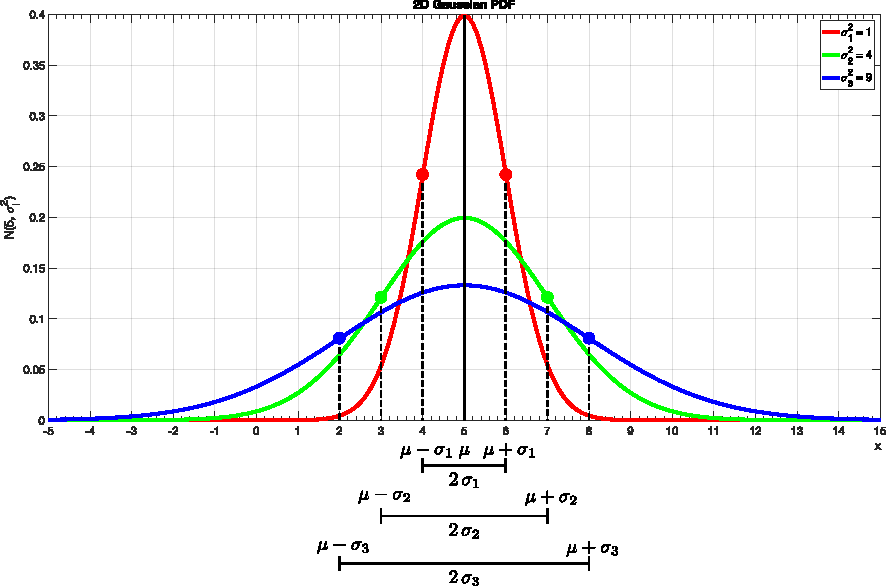
\includegraphics[scale=0.95]{../FIGURES/fig04}
\end{figure}

The term $\mu$ is called mean,. The mean value is the value of the
random variable where the Gaussian PDF has its maximum value and it's
also the value around which the remaining values of that random variable
are distributed.

The quadratic form $\left(\frac{x \, - \, \mu}{\sigma}\right)^2$
represents a straight segment centered at the mean that contains all
the values of the random variable $x$ that gives a value greater
or equal to $K_0$ in the Gaussian PDF.\begin{align*}
\frac{1}{ \sqrt{2 \, \pi} \, \sigma } \, \cdot \, e^{-\frac{1}{2} \, \cdot \, \left(\frac{x \, - \, \mu}{\sigma}\right)^2} \, \geq \, K_0
\end{align*}

\begin{align*}
e^{-\frac{1}{2} \, \cdot \, \left(\frac{x \, - \, \mu}{\sigma}\right)^2} \, &\geq \, K_0 \, \cdot \, \sqrt{2 \, \pi} \, \sigma\\
-\frac{1}{2} \, \cdot \, \left(\frac{x \, - \, \mu}{\sigma}\right)^2 \, &\geq \, ln \left(K_0 \, \cdot \, \sqrt{2 \, \pi} \, \sigma\right)\\
\left(\frac{x \, - \, \mu}{\sigma}\right)^2 \, &\leq \, -2 \, \cdot \, ln \left(K_0 \, \cdot \, \sqrt{2 \, \pi} \, \sigma\right)\\
\left(\frac{x \, - \, \mu}{\sigma}\right)^2 \, &\leq \, ln \left(K_0 \, \cdot \, \sqrt{2 \, \pi} \, \sigma\right)^{-2}\\
\left(\frac{x \, - \, \mu}{\sigma}\right)^2 \, &\leq \, ln\left(\frac{1}{\left(K_0 \, \cdot \, \sqrt{2 \, \pi} \, \sigma\right)^{2}} \right)\\
\left(\frac{x \, - \, \mu}{\sigma}\right)^2 \, &\leq \, ln\left(\frac{1}{K_0^2 \, \cdot \, 2 \, \pi \, \sigma^2} \right)
\end{align*}

Let's call $K$ to the term $ln\left(\frac{1}{K_0^2 \, \cdot \, 2 \, \pi \, \sigma^2} \right)$
for simplicity.\begin{align*}
\left(\frac{x \, - \, \mu}{\sigma}\right)^2 \, &\leq \, K\\
\left(x \, - \, \mu \right)^2 \, &\leq \, K \, \sigma^2\\
\pm \, \left(x \, - \, \mu \right) \, &\leq \, K \, \sigma\\
\end{align*}
\begin{center}
$\mu \, - \, K \, \sigma \, \leq \, x  \, \leq \, \mu \, + \, K \, \sigma ~ \longrightarrow ~ \text{size} \, = \, 2\,K\,\sigma$
\par\end{center}

\begin{align*}
Pr\left( a \, \leq \, x  \, \leq \, b \right) \, = \, \int_{a}^{b} \mathcal{N}\left(\mu, \, \sigma^2\right) \, = \, \frac{1}{\sqrt{2 \, \pi} \, \sigma}\int_a^b e^{\frac{-(x-\mu)^2}{2\sigma^2}} \, dx
\end{align*}

The error function is defined as:

\begin{align*}
\mbox{erf}\left(x\right) \, = \, \frac{1}{\sqrt{\pi}}\int_{-x}^{x} e^{-t^2} \, dt \, = \, \frac{2}{\sqrt{\pi}}\int_{0}^{x} e^{-t^2} \, dt
\end{align*}

\begin{align*}
Pr\left( a \, \leq \, x  \, \leq \, b \right) \, &= \, \frac{1}{\sqrt{2 \, \pi} \, \sigma}\int_a^b e^{\frac{-(x-\mu)^2}{2\sigma^2}}\ dx \, =\\
&= \, \frac{1}{\sqrt{2 \, \pi} \, \sigma}\int_a^b e^{- \left(\frac{x \, - \, \mu}{\sqrt{2} \, \sigma}\right)^2}\ dx \, =\\
&= \, \frac{1}{\sqrt{2 \, \pi} \, \sigma} \left(\int_0^b e^{- \left(\frac{x \, - \, \mu}{\sqrt{2} \, \sigma}\right)^2}\ dx \, - \, \int_0^a e^{- \left(\frac{x \, - \, \mu}{\sqrt{2} \, \sigma}\right)^2} \, dx\right) \, =\\
&= \, \frac{1}{\sqrt{2 \, \pi} \, \sigma} \, \int_0^b e^{- \left(\frac{x \, - \, \mu}{\sqrt{2} \, \sigma}\right)^2}\ dx \, - \, \frac{1}{\sqrt{2 \, \pi} \, \sigma} \, \int_0^a e^{- \left(\frac{x \, - \, \mu}{\sqrt{2} \, \sigma}\right)^2} \, dx
\end{align*}

Let's change the integration variable:

\begin{align*}
t \, &= \, \left(\frac{x \, - \, \mu}{\sqrt{2} \, \sigma}\right)\\
dt \, &= \, \frac{1}{\sqrt{2} \, \sigma} \, dx\\
dx \, &= \, \sqrt{2} \, \sigma \, dt
\end{align*}

\begin{align*}
x \, &= \,  b ~ \longrightarrow \, t \, = \, \left(\frac{b \, - \, \mu}{\sqrt{2} \, \sigma}\right)\\
x \, &= \,  a ~ \longrightarrow \, t \, = \, \left(\frac{a \, - \, \mu}{\sqrt{2} \, \sigma}\right)
\end{align*}

\begin{align*}
Pr\left( a \, \leq \, x  \, \leq \, b \right) \, &= \, \frac{1}{\sqrt{2 \, \pi} \, \sigma}\int_a^b e^{\frac{-(x-\mu)^2}{2\sigma^2}}\ dx \, = \,\\
&= \, \frac{1}{\sqrt{2 \, \pi} \, \sigma} \, \int_0^b e^{- \left(\frac{x \, - \, \mu}{\sqrt{2} \, \sigma}\right)^2}\ dx \, - \, \frac{1}{\sqrt{2 \, \pi} \, \sigma} \, \int_0^a e^{- \left(\frac{x \, - \, \mu}{\sqrt{2} \, \sigma}\right)^2} \, dx \, =\\
&= \, \frac{\sqrt{2}\,\sigma}{\sqrt{2 \, \pi} \, \sigma} \, \int_0^{\left(\frac{b \, - \, \mu}{\sqrt{2} \, \sigma}\right)} e^{- t^2}\ dt \, - \, \frac{\sqrt{2}\,\sigma}{\sqrt{2 \, \pi} \, \sigma} \, \int_0^{\left(\frac{a \, - \, \mu}{\sqrt{2} \, \sigma}\right)} e^{- t^2} \, dx \, =\\
&= \, \frac{1}{\sqrt{\pi}} \, \int_0^{\left(\frac{b \, - \, \mu}{\sqrt{2} \, \sigma}\right)} e^{- t^2}\ dt \, - \, \frac{1}{\sqrt{\pi}} \, \int_0^{\left(\frac{a \, - \, \mu}{\sqrt{2} \, \sigma}\right)} e^{- t^2} \, dt
\end{align*}

\begin{align*}
\frac{1}{\sqrt{\pi}} \, \int_0^{\left(\frac{b \, - \, \mu}{\sqrt{2} \, \sigma}\right)} e^{- t^2}\ dt \, &= \, \frac{2}{2} \, \frac{1}{\sqrt{\pi}} \, \int_0^{\left(\frac{b \, - \, \mu}{\sqrt{2} \, \sigma}\right)} e^{- t^2}\ dt \, = \, \frac{1}{2}\,\text{erf}\left(\frac{b \, - \, \mu}{\sqrt{2} \, \sigma}\right)\\
\frac{1}{\sqrt{\pi}} \, \int_0^{\left(\frac{a \, - \, \mu}{\sqrt{2} \, \sigma}\right)} e^{- t^2}\ dt \, &= \, \frac{2}{2} \, \frac{1}{\sqrt{\pi}} \, \int_0^{\left(\frac{a \, - \, \mu}{\sqrt{2} \, \sigma}\right)} e^{- t^2}\ dt \, = \, \frac{1}{2}\,\text{erf}\left(\frac{a \, - \, \mu}{\sqrt{2} \, \sigma}\right)
\end{align*}

\begin{align*}
Pr\left( a \, \leq \, x  \, \leq \, b \right) \, = \, \frac{1}{2}\left[\text{erf}\left(\frac{b-\mu}{\sqrt{2}\sigma}\right)-\text{erf}\left(\frac{a-\mu}{\sqrt{2}\sigma}\right)\right]
\end{align*}

\begin{align*}
Pr\left( \mu \, - \, K \, \sigma \, \leq \, x  \, \leq \, \mu \, + \, K \, \sigma \right) \, = \, \frac{1}{2}\left[\text{erf}\left(\frac{K}{\sqrt{2}}\right)-\text{erf}\left(\frac{-K}{\sqrt{2}}\right)\right]
\end{align*}

\begin{align*}
\text{erf}\left(-x\right) \, = \, -\,\text{erf}\left(x\right)
\end{align*}

\begin{align*}
Pr\left( \mu \, - \, K \, \sigma \, \leq \, x  \, \leq \, \mu \, + \, K \, \sigma \right) \, = \, \text{erf}\left(\frac{K}{\sqrt{2}}\right)
\end{align*}

\begin{align*}
K \, &= \, 1 ~ \longrightarrow \, Pr\left(\mu \, - \, 1\,\sigma \, \leq \, x \, \leq \, \mu \, + \, 1\,\sigma\right) \, = \, \text{erf}\left(\frac{1}{\sqrt{2}}\right) \, = \, 0.682689 ~ \left(68.269\%\right)\\
K \, &= \, 2 ~ \longrightarrow \, Pr\left(\mu \, - \, 2\,\sigma \, \leq \, x \, \leq \, \mu \, + \, 2\,\sigma\right) \, = \, \text{erf}\left(\frac{2}{\sqrt{2}}\right) \, = \, 0.954499 ~ \left(95.450\%\right)\\
K \, &= \, 3 ~ \longrightarrow \, Pr\left(\mu \, - \, 3\,\sigma \, \leq \, x \, \leq \, \mu \, + \, 3\,\sigma\right) \, = \, \text{erf}\left(\frac{3}{\sqrt{2}}\right) \, = \, 0.997300 ~ \left(99.730\%\right)
\end{align*}

\begin{figure}[H]
\centering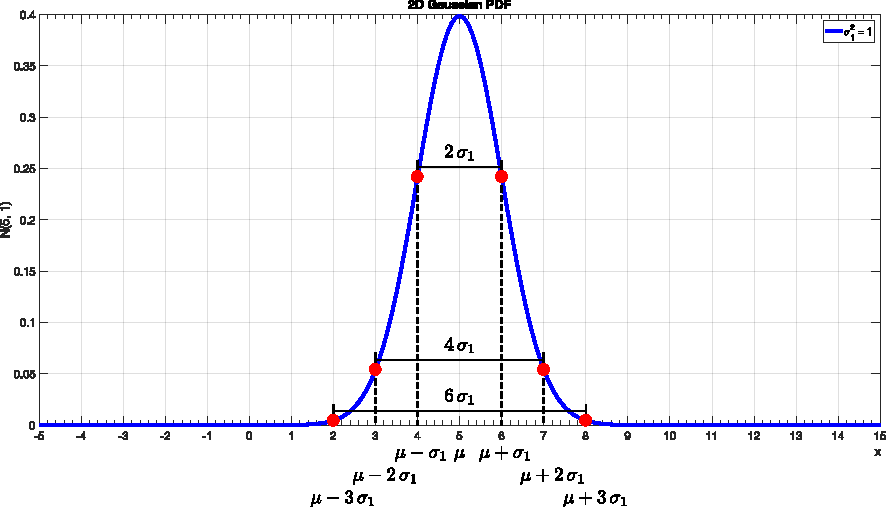
\includegraphics[scale=0.95]{../FIGURES/fig05}
\end{figure}

\textbf{Multivariate Gaussian probability density function.}

The term $\vec{x}$ is a real vector with N dimensions.

\begin{align*}
\vec{x} \, = \, \begin{pmatrix} x_1\\ x_2\\ \vdots\\ x_j\\ \vdots\\ x_N \end{pmatrix} \, \in \, \mathbb{R}^{N \times 1}
\end{align*}:

\begin{align*}
p\left(\vec{x}\right) \, = \, \mathcal{N}\left(\vec{\mu}, \Sigma\right) \, = \, \frac{1}{ \left(2\,\pi \right)^{N/2} \, \begin{vmatrix} \Sigma \end{vmatrix}^{1/2} } \, \cdot \, e^{-\frac{1}{2} \, \cdot \, \left(\vec{x} \, - \, \vec{\mu} \right)^T \, \cdot \, \Sigma^{-1} \, \cdot \, \left(\vec{x} \, - \, \vec{\mu}\right) }
\end{align*}

where the normalizing constant $\frac{1}{ \left(2\,\pi \right)^{N/2} \, \begin{vmatrix} \Sigma \end{vmatrix}^{1/2} }$
makes the volume under the multivariate Gaussian PDF equal to 1.

\begin{align*}
0 \, \leq \, \mathcal{N}\left(\vec{\mu}, \, \Sigma\right) \, \leq \, \infty
\end{align*}

\begin{align*}
0 \, \leq \, \frac{1}{ \left(2\,\pi \right)^{N/2} \, \begin{vmatrix} \Sigma \end{vmatrix}^{1/2} } \, \cdot \, e^{-\frac{1}{2} \, \cdot \, \left(\vec{x} \, - \, \vec{\mu}\right)^T \, \cdot \, \Sigma^{-1} \, \cdot \, \left(\vec{x} \, - \, \vec{\mu}\right) } \, \leq \, \infty
\end{align*}

The vector $\vec{\mu}$ is called mean. The mean vector $\vec{\mu}$
is a real vector with N dimensions. The mean vector $\vec{\mu}$ is
the value of the random vector $\vec{x}$ where the Multivariate Gaussian
PDF has its maximum value and it's also the value around which the
remaining values of that random vector $\vec{x}$ are distributed.

\begin{align*}
\vec{\mu} \, = \, \begin{pmatrix}\mu_1\\\mu_2\\ \vdots\\ \mu_j\\ \vdots\\ \mu_N \end{pmatrix} \in \, \mathbb{R}^{N \times 1}
\end{align*}

The matrix $\Sigma$ is called covariance matrix. The covariance matrix
$\Sigma$ is a real symmetric matrix with N dimensions. $\Sigma \, \in \, \mathbb{R}^{N \times N}$.
Obviously, all the variances and covariances of the covariance matrix
$\Sigma$ are positive:

\begin{align*}
\sigma_i^2 \, \geq \, 0, ~ &\forall ~ i\, = \, \lbrace 1, \, \ldots\, N \rbrace\\
\sigma_{ij} \, \geq \, 0 ~ &\forall ~ i\, = \, \lbrace 1, \, \ldots\, N \rbrace, \forall ~ j\, = \, \lbrace 1, \, \ldots\, N \rbrace, \, i \, \neq \, j
\end{align*}
\begin{center}
\emph{Note that we haven't defined what are the relations among theses
variances and covariances yet. We will back to this issue later when
we have explained something else.}
\par\end{center}

\begin{align*}
\Sigma \, = \, \begin{pmatrix} 
\sigma_{x_1}^2 & \sigma_{x_1x_2} & \ldots & \sigma_{x_1x_j} & \ldots & \sigma_{x_1x_N}\\
\sigma_{x_1x_2} & \sigma_{x_2}^2 & \ldots & \sigma_{x_2x_j} & \ldots & \sigma_{x_2x_N}\\
\vdots & \vdots & \ddots & \vdots & \vdots & \vdots\\
\sigma_{x_1x_j} & \sigma_{x_2x_j} & \ldots & \sigma_{x_j}^2 & \ldots & \sigma_{x_jx_N}\\
\vdots & \vdots & \vdots & \vdots & \ddots & \vdots\\
\sigma_{x_1x_N} & \sigma_{x_2x_N} & \ldots & \sigma_{x_jx_N} & \ldots & \sigma_{x_N}^2\\
\end{pmatrix}
\end{align*}

Let's talk about the covariance matrix $\Sigma$. Since the covariance
matrix $\Sigma$ is symmetric and real \textbf{the spectral descomposition
theorem} stands that:

Any real symmetric matrix $\Sigma$, with dimensions $N \times N$,
can be written as:

\begin{align*}
\Sigma \, = \, U \, \cdot \, D \, \cdot \, U^T
\end{align*}

where:
\begin{itemize}
\item The matrix $D$ is a real diagonal matrix, with dimensions $N \times N$,
where the entries of the matrix $D$ are the eigenvalues of the matrix
$\Sigma$.\begin{align*}
D \, &= \, 
\begin{pmatrix}
\lambda_1 & 0 & \ldots & 0  & \ldots & 0\\
0 & \lambda_2 & \ldots & 0  & \ldots & 0\\
\vdots & \vdots & \ddots & \vdots  & \vdots & \vdots\\
0 & 0 & \ldots & \lambda_j  & \ldots & 0\\
\vdots & \vdots & \vdots & \vdots  & \ddots & \vdots\\
0 & 0 & \ldots & 0  & \ldots & \lambda_N\\
\end{pmatrix}
\end{align*}\\
Note: The matrix $\Sigma$ has $N$ eigenvalues. Not all the $N$
eigenvalues are necessarily unique. Some of them might be repeated.
It's fine.
\item The matrix $U$ is a real orthonormal matrix, with dimensions $N \times N$,
whose columns are the eigenvectors of the matrix $\Sigma$.\begin{align*}
U \, = \, \begin{pmatrix}
| & | &  & | &  & |\\
\vec{u}_1 & \vec{u}_2 & \ldots & \vec{u}_j & \ldots & \vec{u}_N\\
| & | &  & | &  & |
\end{pmatrix}
\end{align*}\begin{align*}
U^T \, &= \, U^{-1} ~ \longrightarrow ~ U^T \, \cdot \, U \, = \, I ~ \longrightarrow  ~ \left\{\begin{aligned} \langle \vec{u}_j, \, \vec{u}_k \rangle \, &= \, \vec{u}_j^{\,T} \, \cdot \, \vec{u}_k \, = \, 0, \text{ for }  j \, \neq \, k\\ \langle \vec{u}_j, \, \vec{u}_k \rangle \, &= \, \vec{u}_j^{\,T} \, \cdot \, \vec{u}_k \, = \, 1, \text{ for } j \, = \, k\end{aligned}\right.
\end{align*}\begin{align*}
\Sigma \, \cdot \, \vec{u}_j \, &= \, \lambda_j \, \cdot \, \vec{u}_j, ~ \forall ~ j \, = \, \lbrace 1, \, \ldots, \, N \rbrace
\end{align*}
\end{itemize}
Now, that it has been shown how the matrix $D$ and the matrix $U$
are we can also express the matrix $\Sigma$ as:

\begin{align*}
\Sigma \, &= \, U \, \cdot \, D \, \cdot \, U^T \, =\\
&= \,  \begin{pmatrix}
| & | &  & | &  & |\\
\vec{u}_1 & \vec{u}_2 & \ldots & \vec{u}_j & \ldots & \vec{u}_N\\
| & | &  & | &  & |
\end{pmatrix} \, \cdot \, \begin{pmatrix}
\lambda_1 &  &  &  &  & \\
  & \lambda_2  &  &  &  & \\
  &  & \ddots &  &  & \\
  &  &  & \lambda_j  &  & \\
  &  &  &  & \ddots & \\
  &  &  &  &  & \lambda_N\\
\end{pmatrix} \, \cdot \, \begin{pmatrix}
\text{---} & \vec{u}_1 & \text{---}\\
\text{---} & \vec{u}_2 & \text{---}\\
&\vdots&\\
\text{---} & \vec{u}_j & \text{---}\\
&\vdots&\\
\text{---} & \vec{u}_N & \text{---}\\
\end{pmatrix} \, =\\
&= \, \lambda_1 \, \vec{u}_1 \, \cdot \, \vec{u}_1^{\,T} \, + \, \lambda_2 \, \vec{u}_2 \, \cdot \, \vec{u}_2^{\,T}\, + \, \ldots \, \lambda_j \, \vec{u}_j \, \cdot \, \vec{u}_j^{\,T} \, + \, \ldots \, + \, \lambda_N \, \vec{u}_N \, \cdot \, \vec{u}_N^{\,T}\, =\\
&= \, \sum_{j \, = \, 1}^{N} \lambda_j \, \vec{u}_j \, \vec{u}_j^T
\end{align*}

Let's show the relation between the covariance matrix $\Sigma$ and
its inverse $\Sigma^{-1}$:

\begin{align*}
\Sigma^{-1} \, = \, \left(U \, \cdot \, D \, \cdot \, U^T\right)^{-1} \, = \, \left(U^T\right)^{-1} \, \cdot \, D^{-1} \, \cdot \, U^{-1} \, = \, \left(U^{-1}\right)^{-1} \, \cdot \, D^{-1} \, \cdot \, U^{T} \, = \, U \, \cdot \, D^{-1} \, \cdot \, U^{T}
\end{align*}

Therefore, the matrix $\Sigma^{-1}$, symmetric and real, with dimensions
$N \times N$, can also be described in terms of eigenvalues and enigenvectors.
The eigenvectors of the matrix $\Sigma^{-1}$ are the eigenvectors
of the matrix $\Sigma$. The eigenvalues of the matrix $\Sigma^{-1}$
are the inverse of the eigenvalues of the matrix $\Sigma$. Because
of the matrix $D$ is diagonal it's very easy to calculate it's inverse.

\begin{align*}
D^{-1} \, = \, \begin{pmatrix}
1/\lambda_1 &  &  &  &  & \\
  & 1/\lambda_2  &  &  &  & \\
  &  & \ddots &  &  & \\
  &  &  & 1/\lambda_j  &  & \\
  &  &  &  & \ddots & \\
  &  &  &  &  & 1/\lambda_N\\
\end{pmatrix}
\end{align*}

\begin{displaymath}
\Sigma^{-1} \, = \, U \, \cdot \, D^{-1} \, \cdot \, U^{T} \, = \, \sum_{j \, = \, 1}^{N} \frac{1}{\lambda_j} \, \vec{u}_j \, \vec{u}_j^T
\end{displaymath}

The spectral theorem implies that there is a transformation from the
real symmetric matrix $\Sigma^{-1}$ into a real diagonal matrix $D^{-1}$.
Let's explain why the transformation from a real symmetric matrix
into a real diagonal matrix is important.

Every quadratic function with $N$ variables can be expressed as:

\begin{align*}
q\left(\vec{y}\right) \, &= \, \left\langle \vec{y}, ~ A \, \cdot \, \vec{y} \right\rangle \, =\\
&= \, \vec{y}^{\,T} \, \cdot \, A \, \cdot \, \vec{y} \, =\\
&= \, \sum_{j \, = \, 1}^N\sum_{k \, = \, 1}^{N}A_{jk} \, \cdot \, y_j \, \cdot \, y_k
\end{align*}

The formula for $q\left(\vec{y}\right)$ involves $N^2$ terms, and
the variables are typically coupled. However if the matrix $A$ happens
to be a diagonal matrix, then the formula for $q\left(\vec{y}\right)$
simplifies considerably:

\begin{align*}
q\left(\vec{y}\right) \, = \, \sum_{j \, = \, 1}^N A_{jj} y_j^2
\end{align*}

Such a quadratic form is easy to understand: In each coordinate direction
$y_j$ the graph is a parabola, opening upward if $A_{jj} \, > \, 0$
and opening downward if $A_{jj} \, < \, 0$. There is also the degenerate
case $A_{jj} \, = \, 0$, in which case $q$ is constant with respect
to $y_j$ and the graph in that direction is a horizontal line.

The quadratic form

\begin{align*}
\left\langle \left(\vec{x} \, - \, \vec{\mu}\right), ~ \Sigma^{-1} \, \cdot \, \left(\vec{x} \, - \, \vec{\mu}\right) \right\rangle \, = \, \left(\vec{x} \, - \, \vec{\mu}\right)^T \, \cdot \, \Sigma^{-1} \, \cdot \, \left(\vec{x} \, - \, \vec{\mu}\right)
\end{align*} is the squared statistical distance from the vector $\vec{\mu}$
to the vector $\vec{x}$. This squared statistical distance takes
into account the variances and covariances among the components of
the random vector $\vec{x}$. The squared statistical distance $\left(\vec{x} \, - \, \vec{\mu}\right)^T \, \cdot \, \Sigma^{-1} \, \cdot \, \left(\vec{x} \, - \, \vec{\mu}\right)$
is called the \textbf{squared Mahalanobis distance}. The Mahalanobis
distance reduces to the Euclidean distance when the matrix $\Sigma$
is the identity matrix.

Let's do a change of variable:

\begin{align*}
\vec{y} \, = \, \left(\vec{x} \, - \, \vec{\mu}\right)
\end{align*}

\begin{align*}
\left\langle \left(\vec{x} \, - \, \vec{\mu}\right), ~ \Sigma^{-1} \, \cdot \, \left(\vec{x} \, - \, \vec{\mu}\right) \right\rangle \, &= \, \left(\vec{x} \, - \, \vec{\mu}\right)^T \, \cdot \, \Sigma^{-1} \, \cdot \, \left(\vec{x} \, - \, \vec{\mu}\right) \,=\\
&= \, \vec{y}^{\,T} \, \cdot \, \Sigma^{-1} \, \cdot \, \vec{y} \, =\\
&= \, \vec{y}^{\,T} \, \cdot \, U \, \cdot \, D^{-1} \, \cdot \, U^T \, \cdot \, \vec{y} \, =\\
&= \, \left(U^T \, \cdot \, \vec{y}\right)^T \, \cdot \, D^{-1} \, \cdot \, \left(U^T \, \cdot \, \vec{y}\right) \,=\\
&= \, \left\langle \left(U^T \, \cdot \, \vec{y}\right), ~ D^{-1} \, \cdot \, \left(U^T \, \cdot \, \vec{y}\right) \right\rangle
\end{align*}

\begin{align*}
\begin{pmatrix}
\alpha_{1}\\
\alpha_{2}\\
\vdots\\
\alpha_{j}\\
\vdots\\
\alpha_{N}
\end{pmatrix} \, = \, U^{T} \, \cdot \, \vec{y} \, &= \,
\begin{pmatrix}
u_{11} & u_{12} & \ldots & u_{1k}  & \ldots & u_{1N}\\
u_{21} & u_{22} & \ldots & u_{2k}  & \ldots & u_{2N}\\
\vdots & \vdots & \ddots & \vdots  & \vdots & \vdots\\
u_{j1} & u_{j2} & \ldots & u_{jk}  & \ldots & u_{jN}\\
\vdots & \vdots & \vdots & \vdots  & \ddots & \vdots\\
u_{N1} & u_{N2} & \ldots & u_{Nk}  & \ldots & u_{NN}\\
\end{pmatrix} \, \cdot \, \begin{pmatrix}
y_{1}\\
y_{2}\\
\vdots\\
y_{j}\\
\vdots\\
y_{N}\\
\end{pmatrix} \, =\\
&= \, \begin{pmatrix}
\vec{u}_1^{\,T}, ~ \vec{y}\\
\vec{u}_2^{\,T}, ~ \vec{y}\\
\vdots\\
\vec{u}_j^{\,T}, ~ \vec{y}\\
\vdots\\
\vec{u}_N^{\,T}, ~ \vec{y}\\
\end{pmatrix} \, = \,
\begin{pmatrix}
\left\langle \vec{u}_1, ~ \vec{y} \right\rangle\\
\left\langle \vec{u}_2, ~ \vec{y} \right\rangle\\
\vdots\\
\left\langle \vec{u}_j, ~ \vec{y} \right\rangle\\
\vdots\\
\left\langle \vec{u}_N, ~ \vec{y} \right\rangle
\end{pmatrix}
\end{align*}

\begin{align*}
\left(U^T \, \cdot \, \vec{y}\right)^T \, \cdot \, D^{-1} \, \cdot \, \left(U^T \, \cdot \, \vec{y}\right)
\end{align*}

\begin{align*}
\begin{pmatrix} 
\alpha_1, \, \ldots, \alpha_j, \, \ldots, \, \alpha_N \end{pmatrix} \, \cdot \, \begin{pmatrix} 1/\lambda_1 & & & & & \\ & & \ddots & & & \\ & & & 1/\lambda_j & & \\ & & & & \ddots & \\ & & & & & 1/\lambda_N\\ \end{pmatrix} \, \cdot \, \begin{pmatrix}
\alpha_{1}\\
\vdots\\
\alpha_{j}\\
\vdots\\
\alpha_{N}
\end{pmatrix}
\end{align*}

\begin{align*}
\begin{pmatrix} \frac{1}{\lambda_1} \, \alpha_1, \, \ldots, \frac{1}{\lambda_j} \, \alpha_j, \, \ldots, \, \frac{1}{\lambda_N} \alpha_N \end{pmatrix} \, \cdot \, \begin{pmatrix}
\alpha_{1}\\
\vdots\\
\alpha_{j}\\
\vdots\\
\alpha_{N}
\end{pmatrix}
\end{align*}

\begin{align*}
\frac{1}{\lambda_1} \, \alpha_1^2 \, + \, \ldots \, + \, \frac{1}{\lambda_j} \, \alpha_j^2 \, + \, \ldots \, + \, \frac{1}{\lambda_N} \alpha_N^2 \, = \, \sum_{j \, = \, 1}^{N} \frac{1}{\lambda_j} \, \cdot \, \alpha_j^2
\end{align*}

\begin{align*}
\left\langle \left(\vec{x} \, - \, \vec{\mu}\right), ~ \Sigma^{-1} \, \cdot \, \left(\vec{x} \, - \, \vec{\mu}\right) \right\rangle \, = \, \left(\vec{x} \, - \, \vec{\mu}\right)^T \, \cdot \, \Sigma^{-1} \, \cdot \, \left(\vec{x} \, - \, \vec{\mu}\right) \, &= \, \sum_{j \, = \, 1}^{N} \frac{1}{\lambda_j} \, \cdot \, \alpha_j^2 \,=\\
&= \, \sum_{j \, = \, 1}^{N} \frac{1}{\lambda_j} \, \cdot \, \left\langle \vec{u}_j, \, \left(\vec{x} \, - \, \vec{\mu}\right) \right\rangle^2 \, =\\
&= \, \sum_{j \, = \, 1}^{N} \frac{1}{\lambda_j} \, \cdot \, \left( \vec{u}_j^{\,T} \, \cdot \, \left(\vec{x} \, - \, \vec{\mu}\right) \right)^2
\end{align*}

The term $\alpha_j \, = \, \left\langle \vec{u}_j, \, \left(\vec{x} \, - \, \vec{\mu}\right) \right\rangle \, = \, \vec{u}_j^{\,T} \, \cdot \, \left(\vec{x} \, - \, \vec{\mu}\right)$
represents the $j-th$ coordinate of the vector $\left(\vec{x} \, - \, \vec{\mu}\right)$
in the orthonormal basis $U$. 

Since every real symmetric matrix $A$ has a spectral decomposition
in real eigenvalues and real eigenvectors, this means that every quadratic
function $q\left(\vec{y}\right) \, = \, \left(\vec{y} \, - \, \vec{b}\right)^T \, \cdot \, A \, \cdot \, \left(\vec{y} \, - \, b\right)$
can be expressed as above\\
The set of all the values of the random vector $\vec{x}$ that gives
a constant value $K^2$ in the quadratic function $\left(\vec{x} \, - \, \vec{\mu}\right)^T \, \cdot \, \Sigma^{-1} \, \cdot \, \left(\vec{x} \, - \, \vec{\mu}\right)$
forms a N-dimensional curve. Let's call this set $S$. These N-dimensional
curves also give a constant value $L$ on the Gaussian PDF, that is
why these curves are called contour curves.

\begin{align*}
q\left(\vec{x}\right) \, &= \, \left(\vec{x} \, - \, \vec{\mu}\right)^T \, \cdot \, \Sigma^{-1} \, \cdot \, \left(\vec{x} \, - \, \mu\right) \, = \, \sum_{j \, = \, 1}^{N} \frac{1}{\lambda_j} \, \cdot \, \left( \vec{u}_j^{\,T} \, \cdot \, \left(\vec{x} \, - \, \vec{\mu}\right) \right)^2 \, = \, K^2\\
S \, &= \, \left\lbrace \vec{x}_1, \, \vec{x}_2, \, \ldots  \right\rbrace \text{ forms a N-dimensional curve that solves the above constant expression}\\
p\left(\vec{x}\right) \, &= \, \frac{1}{ \left(2\,\pi \right)^{N/2} \, \begin{vmatrix} \Sigma \end{vmatrix}^{1/2} } \, \cdot \, e^{-\frac{1}{2} \, K^2 } \, = \, L
\end{align*}

For the Gaussian PDF to be well defined, it is necessary for all the
eigenvalues $\lambda_j$ of the covariance matrix $\Sigma$ to be
strictly positive, otherwise the Gaussian PDF cannot be properly normalized.
If all of the eigenvalues $\lambda_j$ are strictly positive, then
these N-dimensional curves have the shape of N-dimensional ellipsoids
with their centres at the vector $\vec{\mu}$, the direction of its
$j-th$ major axis defined by the eigenvector $\vec{u}_j$ of the
covariance matrix $\Sigma$ and with the length of its $j-th$ major
axis defined by $2\,K\,\sqrt{\lambda_j}$.

Summarizing, the covariance matrix $\Sigma$ is a real symmetric matrix,
with dimensions $N \times N$ that can be written in terms of its
$N$ eigenvalues and its $N$ orthonormal eigenvectors using the expression 

\begin{align*}
\Sigma \, = \, \begin{pmatrix} 
\sigma_{x_1}^2 & \sigma_{x_1x_2} & \ldots & \sigma_{x_1x_j} & \ldots & \sigma_{x_1x_N}\\
\sigma_{x_1x_2} & \sigma_{x_2}^2 & \ldots & \sigma_{x_2x_j} & \ldots & \sigma_{x_2x_N}\\
\vdots & \vdots & \ddots & \vdots & \vdots & \vdots\\
\sigma_{x_1x_j} & \sigma_{x_2x_j} & \ldots & \sigma_{x_j}^2 & \ldots & \sigma_{x_jx_N}\\
\vdots & \vdots & \vdots & \vdots & \ddots & \vdots\\
\sigma_{x_1x_N} & \sigma_{x_2x_N} & \ldots & \sigma_{x_jx_N} & \ldots & \sigma_{x_N}^2\\
\end{pmatrix} \, = \, U \, \cdot \, D \, \cdot \, U^T
\end{align*}

and also all its eigenvalues are strictly positive, $\lambda_j \, > \, 0, \, \forall j \, = \, 1, \, \ldots, \, N$

Any real symmetric matrix $A$ with all its eigenvalues strictly positive
is called \textbf{positive definite}. Positive definite matrices are
very important in all kind of contexts for its unique properties.
In any case, I'm not going to write about this properties here because
it's not part the topic of this document.

Therefore, the covariance matrix $\Sigma$ is a positive definite
matrix. So, imagine your are writing a real symmetric matrix $A$
and you want to know if this real symmetric matrix has all its eigenvalues
strictly positive without having to calculate all of them. Well, there
is a test you can do. The test consist on looking at the $N$ upper
left determinants of the matrix $A$, i.e, $\begin{vmatrix}A_j\end{vmatrix}$,
where $A_j$ is the upper left $j \times j$ submatrix. All the eigenvalues
of our real symmetric matrix $A$ will be strictly positive if and
only if $\begin{vmatrix}A_j\end{vmatrix} \, > \, 0, ~ \forall ~ 1 \, \leq \, j \, \leq \, N$

Is the following matrix positive definite?

\begin{align*}
A \, = \, \begin{pmatrix} 
2 & -1 & 0\\
-1 & 2 & -1\\
0 & -1 & 2
\end{pmatrix}
\end{align*}

\begin{align*}
&\begin{vmatrix} A_1 \end{vmatrix} \, = \, 2 \, > \, 0\\
&\begin{vmatrix} A_2 \end{vmatrix} \, = \, \begin{pmatrix} 
2 & -1\\
-1 & 2
\end{pmatrix} \, = \, 2 \, \cdot \, 2 \, - \, \left(-1 \, \cdot \, -1\right) \, = \, 4 \, - \, 1 \, = \, 3 \, > \, 0\\
&\begin{vmatrix} A_3 \end{vmatrix} \, = \, \begin{pmatrix} 
2 & -1 & 0\\
-1 & 2 & -1\\
0 & -1 & 2
\end{pmatrix} \, = \, \left(2 \, \cdot \, 2 \, \cdot \, 2\right) \, + \, \left(-1 \, \cdot \, -1 \, \cdot \, 0\right) \, + \, \left(0 \, \cdot \, -1 \, \cdot \, -1\right) \, -\\
&-\, \begin{pmatrix} \left(0 \, \cdot \, 2 \, \cdot \, 0\right) \, + \, \left(-1 \, \cdot \, -1 \, \cdot \, 2\right) \, + \, \left(2 \, \cdot \, -1 \, \cdot \, -1\right)\end{pmatrix} \, = \, 8 \, - \, \begin{pmatrix} 2 \, + 2 \end{pmatrix} \, = \, 8 \, - \, 4 \, = \, 4 \, > \, 0
\end{align*}

$\begin{vmatrix}A_j\end{vmatrix} \, > \, 0, ~ \forall ~ 1 \, \leq \, j \, \leq \, 3$,
so the matrix $A$ is positive definite.

So, for the matrix $\Sigma$, these constraints of having $\begin{vmatrix}\Sigma_j\end{vmatrix} \, > \, 0, ~ \forall ~ 1 \, \leq \, j \, \leq \, N$
establish some relationships among the variances and covariances that
constitute the matrix $\Sigma$. 

\textbf{Note}: the constraints and conditions that apply to the matrix
$\Sigma$ are the same that the ones that apply to the matrix $\Sigma^{-1}$.
Therefore, we don't have the necessity of analyzing two different
sets of constraints and conditions.

For example:

\begin{align*}
N \, = \, 2 ~ \longrightarrow ~ \Sigma \, = \, \begin{pmatrix}
\sigma_{x_1}^2 & \sigma_{x_1x_2}\\
\sigma_{x_1x_2} & \sigma_{x_2}^2 \,
\end{pmatrix}
\end{align*}

\begin{align*}
\begin{vmatrix} \Sigma_{1}\end{vmatrix} \, = \, \sigma_{x_2}^2 \, > \, 0 \, \longrightarrow \, \begin{vmatrix} \sigma_{x_2} \end{vmatrix} \, > \, 0
\end{align*}

\begin{align*}
\begin{vmatrix} \sigma_{x_2} \end{vmatrix} \, > \, 0 \, \longrightarrow \, \left\{\begin{aligned} \sigma_{x_2} \, > \,0 \, \longrightarrow \, \begin{vmatrix} \sigma_{x_2} \end{vmatrix} \, &= \, \sigma_{x_2} \, > \,0 ~ &\longrightarrow ~ \sigma_{x_2} \, > \,0\\
\sigma_{x_2} \, < \,0 \, \longrightarrow \, \begin{vmatrix} \sigma_{x_2} \end{vmatrix} \, &= \, -\sigma_{x_2} \, > \,0 ~ &\longrightarrow ~ \sigma_{x_2} \, < \,0\end{aligned}\right.
\end{align*}

The condition $\sigma_{x_2} \, < \,0$ is not valid since the standard
deviation is a measure of the dispersion of the data, so it must be
positive, not negative.

When analyzing the $\begin{vmatrix} \sigma_{x_2} \end{vmatrix}$ I
haven't taken into account the value $\sigma_{x_2} \, = \, 0$, only
the value $\sigma_{x_2} \, > \, 0$, because, although a standard
deviation can be 0, this value express that I am working with a deterministic
value, not a random variable. Because of I'm working with random variables
(packed in the form of a vector), i.e, non deterministic values, the
value $\sigma_{x_2} \, = \, 0$ is not considered.

\begin{align*}
\begin{vmatrix} \Sigma_{2} \end{vmatrix} \, = \, \sigma_{x_2}^2 \, \cdot \, \sigma_{x_1}^2 \, - \, \left( \sigma_{x_1x_2} \, \cdot \, \sigma_{x_1x_2}\right) \, = \, \sigma_{x_2}^2 \, \cdot \, \sigma_{x_1}^2 \, - \, \sigma_{x_1x_2}^2 \, > \, 0 
\end{align*}

\begin{align*}
\sigma_{x_2}^2 \, \cdot \, \sigma_{x_1}^2 \, - \, \sigma_{x_1x_2}^2 \, > \, 0 \, \longrightarrow \, \left(\sigma_{x_2} \, \cdot \, \sigma_{x_1}\right)^2 \, > \, \sigma_{x_1x_2}^2 \, \longrightarrow  \, \begin{vmatrix}\sigma_{x_2} \, \cdot \, \sigma_{x_1} \end{vmatrix}  \, > \, \begin{vmatrix} \sigma_{x_1x_2} \end{vmatrix}
\end{align*}

A standard deviation is a measure of the dispersion of the data, therefore,
it must be positive:

\begin{gather*}
\sigma_j \, > \, 0, ~ \forall ~ j \, = \, 1, \, \ldots, \, N\\
(\text{for random variables we only use the symbol >})\\
\sigma_{x_1} \, > \, 0\\
\sigma_{x_2} \, > \, 0\\
(\text{ equal symbol is supressed, due to the above condition})
\end{gather*} \begin{align*}
\sigma_{x_1} \, \cdot \, \sigma_{x_2} \, > \, 0 ~ &\longrightarrow ~ \begin{vmatrix} \sigma_{x_1} \, \cdot \, \sigma_{x_2} \end{vmatrix} \, = \,  \sigma_{x_1} \, \cdot \, \sigma_{x_2}\\
\begin{vmatrix}\sigma_{x_2} \, \cdot \, \sigma_{x_1} \end{vmatrix}  \, > \, \begin{vmatrix} \sigma_{x_1x_2} \end{vmatrix} ~ &\longrightarrow ~ \sigma_{x_1} \, \cdot \, \sigma_{x_2} \, > \, \begin{vmatrix} \sigma_{x_1x_2} \end{vmatrix}
\end{align*}

\begin{align*}
\begin{vmatrix} \sigma_{x_1x_2} \end{vmatrix} \, < \, \sigma_{x_1} \, \cdot \, \sigma_{x_2} \, \longrightarrow \, \left\{\begin{aligned} \sigma_{x_1x_2} \, > \,0, \, \begin{vmatrix} \sigma_{x_1x_2} \end{vmatrix} \, &= \, \sigma_{x_1x_2} \, < \,\sigma_{x_1} \, \cdot \, \sigma_{x_2} \, ~~~\longrightarrow \, \sigma_{x_1x_2} \, < \,\sigma_{x_1} \, \cdot \, \sigma_{x_2}\\
\sigma_{x_1x_2} \, < \,0, \, \begin{vmatrix} \sigma_{x_1x_2} \end{vmatrix} \, &= \, -\,\sigma_{x_1x_2} \, < \,\sigma_{x_1} \, \cdot \, \sigma_{x_2} \, \longrightarrow \, \sigma_{x_1x_2} \, > \,-\,\sigma_{x_1} \, \cdot \, \sigma_{x_2} \end{aligned}\right.
\end{align*}

Finally, the conditions for the matrix $\Sigma$ (and $\Sigma^{-1}$)
to be positive definite are:

\begin{gather*}
\sigma_{x_1} \, > \, 0\\
\sigma_{x_2} \, > \, 0\\
-\,\sigma_{x_1} \, \cdot \, \sigma_{x_2} \, < \, \sigma_{x_1x_2} \, < \, \sigma_{x_1} \, \cdot \, \sigma_{x_2}\\
(\text{Note the lack of the equal symbol})
\end{gather*}

Reorganizing a bit the terms of the last condition I get:

\begin{gather*}
-\,1 \, < \, \frac{\sigma_{x_1x_2}}{\sigma_{x_1} \, \cdot \, \sigma_{x_2}} \, < \, 1\\
(\text{Note the lack of the equal symbol})
\end{gather*}

The correlation coefficient is defined as:

\begin{gather*}
\rho \, = \, \frac{\sigma_{x_1x_2}}{\sigma_{x_1} \, \cdot \, \sigma_{x_2}}\\
-\,1 \, \leq \, \rho \, \leq \, 1\\
(\text{Note the presence of the equal symbol})
\end{gather*}

Basically our conditions stands that I must have strictly positive
standard deviations and a correlation coefficient between $(-\,1, \, 1)$
(open range, therefore the extremes are excluded):

\begin{gather*}
\sigma_{x_1} \, > \, 0\\
\sigma_{x_2} \, > \, 0\\
-\,1 \, < \, \rho \, < \, 1\\
\begin{pmatrix} -\,\sigma_{x_1} \, \cdot \, \sigma_{x_2} \, < \, \sigma_{x_1x_2} \, < \, \sigma_{x_1} \, \cdot \, \sigma_{x_2}\\
\text{Note the lack of the equal symbol}
\end{pmatrix}
\end{gather*}

\newpage

Let's study the bivariate Gaussian PDF. The covariance matrix $\Sigma$
is a positive definite matrix with dimension $N \times N$. This means
that the covariance matrix $\Sigma$ is a real symmetric matrix, with
dimension $N \times N$, with $N$ real eigenvalues that are strictly
positive, $\lambda_j \, > \, 0 ~ \forall ~ j \, = \, 1, \, \ldots, \, N$,
due to the constraints:

\begin{gather*}
\sigma_{x_1} \, > \, 0\\
\sigma_{x_2} \, > \, 0\\
-\,1 \, < \, \rho \, < \, 1\\
\begin{pmatrix} -\,\sigma_{x_1} \, \cdot \, \sigma_{x_2} \, < \, \sigma_{x_1x_2} \, < \, \sigma_{x_1} \, \cdot \, \sigma_{x_2}\\
\text{Note the lack of the equal symbol}
\end{pmatrix}
\end{gather*}

and with $N$ orthonormal eigenvectors, $U^T \, = \, U^{-1} ~ \longrightarrow ~ U^{T} \, \cdot \, U \, = \, I$.

\begin{align*}
\Sigma \, = \, 
\begin{pmatrix} 
\sigma_{x_1}^2 & \sigma_{x_1x_2}\\
\sigma_{x_1x_2} & \sigma_{x_2}^2
\end{pmatrix} \, = \, U \, \cdot \, D \, \cdot \, U^T \, = \, \begin{pmatrix}
u_{11} & u_{21}\\
u_{12} & u_{22}
\end{pmatrix} \, \cdot \, \begin{pmatrix}
\lambda_1 &  0\\
0  & \lambda_2
\end{pmatrix} \, \cdot \, \begin{pmatrix}
u_{11} & u_{12}\\
u_{21} & u_{22}
\end{pmatrix} \, = \, \sum_{j \, = \, 1}^{2}\lambda_j \, \vec{u}_j \, \vec{u}_j^{\,T}
\end{align*}

Besides, the matrix $\Sigma^{-1}$ is also a positive definite matrix
with dimension $N \times N$. As before, this means that the matrix
$\Sigma^{-1}$ is a real symmetric matrix, with dimension $N \times N$,
with $N$ real eigenvalues that are strictly positive, $1/\lambda_j \, > \, 0 ~ \forall ~ j \, = \, 1, \, \ldots, \, N$,
due to the constraints:

\begin{gather*}
\sigma_{x_1} \, > \, 0\\
\sigma_{x_2} \, > \, 0\\
-\,1 \, < \, \rho \, < \, 1\\
\begin{pmatrix} -\,\sigma_{x_1} \, \cdot \, \sigma_{x_2} \, < \, \sigma_{x_1x_2} \, < \, \sigma_{x_1} \, \cdot \, \sigma_{x_2}\\
\text{Note the lack of the equal symbol}
\end{pmatrix}
\end{gather*}

and with $N$ orthonormal eigenvectors, $U^T \, = \, U^{-1} ~ \longrightarrow ~ U^{T} \, \cdot \, U \, = \, I$.

\begin{align*}
\Sigma^{-1} \, &= \, \frac{1}{\begin{vmatrix} \Sigma \end{vmatrix}} 
\begin{pmatrix}
\sigma_{x_2}^2 & -\,\sigma_{x_1x_2}\\
-\,\sigma_{x_1x_2} & \sigma_{x_1}^2 \,
\end{pmatrix} \, = \, \frac{1}{\sigma_{x_1}^2 \, \sigma_{x_2}^2 \, - \, \sigma_{x_1x_2}^2}
\begin{pmatrix} 
\sigma_{x_2}^2 & -\,\sigma_{x_1x_2}\\
-\,\sigma_{x_1x_2} & \sigma_{x_1}^2
\end{pmatrix} \,=\\
&= \, U \, \cdot \, D^{-1}\, \cdot \, U^T \, = \, \begin{pmatrix}
u_{11} & u_{21}\\
u_{12} & u_{22}
\end{pmatrix} \, \cdot \, \begin{pmatrix}
1/\lambda_1 &  0\\
0  & 1/\lambda_2
\end{pmatrix} \, \cdot \, \begin{pmatrix}
u_{11} & u_{12}\\
u_{21} & u_{22}
\end{pmatrix} \, =\\
&=\, \sum_{j \, = \, 1}^{2}\frac{1}{\lambda_j} \, \vec{u}_j \, \vec{u}_j^{\,T}
\end{align*}

The quadratic function\begin{align*}
\left(\vec{x} \, - \, \vec{\mu}\right)^T \, \cdot \, \Sigma^{-1} \, \cdot \, \left(\vec{x} \, - \, \vec{\mu}\right) \, = \, K^2
\end{align*}

represents a 2D ellipse with its center located at the vector $\vec{\mu}$,
the directions of its principal axes defined by the orthonormal eigenvectors
of the covariance matrix $\Sigma$, $\vec{u}_1$ and $\vec{u}_2$,
and with the length of its principal axes defined by $2\,K \, \sqrt{\lambda_j}$.

\begin{figure}[H]
\centering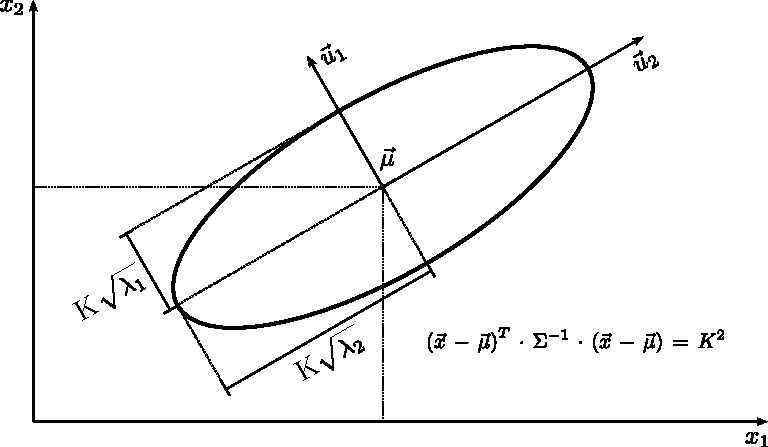
\includegraphics[scale=0.95]{../FIGURES/fig07}
\end{figure}

The quadratic function $\left(\vec{x} \, - \, \vec{\mu}\right)^T \, \cdot \, \Sigma^{-1} \, \cdot \, \left(\vec{x} \, - \, \vec{\mu}\right)$
can be express in two ways:

\begin{align*}
\left(\vec{x} \, - \, \vec{\mu}\right)^T \, \cdot \, \Sigma^{-1} \, \cdot \, \left(\vec{x} \, - \, \vec{\mu}\right) \, &= \, \frac{1}{\begin{vmatrix} \Sigma \end{vmatrix}} \, \cdot \, \begin{pmatrix}x_1 \, - \, \mu_1, x_2 \, - \, \mu_2 \end{pmatrix} \, \cdot \,
\begin{pmatrix} 
\sigma_{x_2}^2 & -\,\sigma_{x_1x_2}\\
-\,\sigma_{x_1x_2} & \sigma_{x_1}^2
\end{pmatrix} \, \cdot \, \begin{pmatrix}x_1 \, - \, \mu_1\\ x_2 \, - \, \mu_2 \end{pmatrix} \, =\\
&= \, \frac{1}{\begin{vmatrix} \Sigma \end{vmatrix}} \, \cdot \, \begin{pmatrix} \sigma_{x_2}^2 \, \left(x_1 \, - \, \mu_1\right)^2 \, + \, \sigma_{x_1}^2 \, \left(x_2 \, - \, \mu_2\right)^2 \, - \, 2\,\sigma_{x_1x_2} \, \left(x_1 \, - \, \mu_1\right) \, \left(x_2 \, - \, \mu_2\right)\end{pmatrix}\\
\left(\vec{x} \, - \, \vec{\mu}\right)^T \, \cdot \, \Sigma^{-1} \, \cdot \, \left(\vec{x} \, - \, \vec{\mu}\right) \, &= \, \sum_{j \, = \, 1}^{2} \frac{1}{\lambda_j} \, \cdot \, \left( \vec{u}_j^{\,T} \, \cdot \, \left(\vec{x} \, - \, \vec{\mu}\right) \right)^2 \,=\\
&= \, \left(\frac{u_{11}^2}{\lambda_1} + \frac{u_{21}^2}{\lambda_2}\right)\,\cdot\,\left(x_1 \, - \, \mu_1\right)^2 \, + \, \left(\frac{u_{12}^2}{\lambda_1} + \frac{u_{22}^2}{\lambda_2}\right)\,\cdot\,\left(x_2 \, - \, \mu_2\right)^2 \, +\\
&\, + \, 2\,\cdot\,\left(\frac{u_{11}\,\cdot\,u_{12}}{\lambda_1} + \frac{u_{21}\,\cdot\,u_{22}}{\lambda_2}\right)\,\cdot\,\left(x_1 \, - \, \mu_1\right)\,\cdot\,\left(x_2 \, - \, \mu_2\right)
\end{align*}

\begin{align*}
Pr\left( \vec{x} \in \text{ ellipse of } K \, = \, 1\right) \, = \, 0.682689 ~ \left(68.269\%\right)\\
Pr\left( \vec{x} \in \text{ ellipse of } K \, = \, 2\right) \, = \, 0.954499 ~ \left(95.450\%\right)\\
Pr\left( \vec{x} \in \text{ ellipse of } K \, = \, 3\right) \, = \, 0.997300 ~ \left(99.730\%\right)
\end{align*}

Let's describe how to calculate the eigenvalues and the eigenvectors
of the matrix $\Sigma$. 

If the following expression can be written:

\begin{align*}
\Sigma \, \cdot \, \vec{u}_j \, = \, \lambda_j \, \cdot \, \vec{u}_j
\end{align*}

then value $\lambda_j$ is an eigenvalue of the matrix $\Sigma$ and
the vector $\vec{u}_j$ is an eigenvector of the matrix $\Sigma$
that are associated.

Therefore, if the above equation is satisfied, then the equation can
be written as:

\begin{align*}
\Sigma \, \cdot \, \vec{u}_j \, - \, \lambda_j \, \cdot \, \vec{u}_j \, = \, \left(\Sigma \, - \, \lambda_j \, I \right) \, \cdot \, \vec{u}_j \, = \, 0
\end{align*}

The equation $\left(\Sigma \, - \, \lambda_j \, I \right) \, \cdot \, \vec{u}_j \, = \, 0$
has a non-zero solution, $\vec{u}_j \, \neq \, 0$, if and only if
$\begin{vmatrix}\Sigma \, - \, \lambda_j \, I\end{vmatrix} \, = \, 0$.
Therefore, the eigenvalues of the covariance matrix $\Sigma$ are
the roots of the equation $\begin{vmatrix} \Sigma \, - \, \lambda_j \, I\end{vmatrix} \, = \, 0$.
The values $\lambda_j$ obtained are introduced in the expression
$\left(\Sigma \, - \, \lambda_j \, I \right) \, \cdot \, \vec{u}_j \, = \, 0$
to calculate the eigenvectors $\vec{u}_j$.

We are going to use the relation:

\begin{gather*}
\rho = \frac{\sigma_{x_1x_2}}{\sigma_{x_1} \, \sigma_{x_2}}\\
-1 \, < \, \rho \, < \, 1\\
\begin{pmatrix}\text{Note the lack of the equal symbol due to our conditions for the matrices } \Sigma \text{ and } \Sigma^{-1} \text{ to be posititive definite}\end{pmatrix}
\end{gather*}

\begin{align*}
\begin{vmatrix}
 \Sigma \, - \, \lambda_j \, I
\end{vmatrix} \, &= \,
\begin{vmatrix}
\begin{pmatrix} 
\sigma_{x_1}^2 & \sigma_{x_1x_2}\\
\sigma_{x_1x_2} & \sigma_{x_2}^2
\end{pmatrix} \, - \, \begin{pmatrix} 
\lambda_j & 0\\
0 & \lambda_j
\end{pmatrix}
\end{vmatrix} \, = \, \begin{vmatrix}
\begin{pmatrix} 
\sigma_{x_1}^2 \, - \, \lambda_j & \sigma_{x_1x_2}\\
\sigma_{x_1x_2} & \sigma_{x_2}^2 \, - \, \lambda_j
\end{pmatrix}
\end{vmatrix} \,=\\
&= \, \left(\sigma_{x_1}^2 \, - \, \lambda_j\right) \, \left(\sigma_{x_2}^2 \, - \, \lambda_j\right) \, - \, \sigma_{x_1x_2}^2 \, =\\
&= \, \left(\sigma_{x_1}^2 \, - \, \lambda_j\right) \, \left(\sigma_{x_2}^2 \, - \, \lambda_j\right) \, - \, \rho^2\sigma_{x_1}^2\sigma_{x_2}^2 \, =\\
&= \lambda_j^2 \, - \, \left(\sigma_{x_1}^2 \, + \, \sigma_{x_2}^2\right) \, \lambda_j \, + \, \sigma_{x_1}^2 \, \sigma_{x_2}^2 \, \left(1 \, - \, \rho^2\right) \, = \, 0
\end{align*}

\begin{align*}
\lambda_1 \, &= \, \frac{1}{2}\begin{pmatrix}\sigma_{x_1}^2 \, + \, \sigma_{x_2}^2 \, + \, \sqrt{\left(\sigma_{x_1}^2 \, + \, \sigma_{x_2}^2\right)^2 \, - \, 4\,\sigma_{x_1}^2 \, \sigma_{x_2}^2 \, \left(1 \, - \, \rho^2\right)}\end{pmatrix}\\
\lambda_2 \, &= \, \frac{1}{2}\begin{pmatrix}\sigma_{x_1}^2 \, + \, \sigma_{x_2}^2 \, - \, \sqrt{\left(\sigma_{x_1}^2 \, + \, \sigma_{x_2}^2\right)^2 \, - \, 4\,\sigma_{x_1}^2 \, \sigma_{x_2}^2 \, \left(1 \, - \, \rho^2\right)}\end{pmatrix}
\end{align*}

Now, I calculate the eigenvectors $\vec{u}_j$:

\begin{gather*}
\Sigma \, \cdot \, \vec{u}_1 \, = \, \lambda_1 \, \vec{u}_1
\end{gather*}

\begin{align*}
&\begin{pmatrix} 
\sigma_{x_1}^2 & \sigma_{x_1x_2}\\
\sigma_{x_1x_2} & \sigma_{x_2}^2
\end{pmatrix} \, \cdot \, \begin{pmatrix} u_{11}\\ u_{12} \end{pmatrix} \, = \, \lambda_1 \, \begin{pmatrix}u_{11}\\u_{12} \end{pmatrix}\\\\
&\begin{pmatrix}
\sigma_{x_1}^2 & \sigma_{x_1x_2}\\
\sigma_{x_1x_2} & \sigma_{x_2}^2
\end{pmatrix} \, \cdot \, \begin{pmatrix} u_{11}\\ u_{12} \end{pmatrix} \, - \, \lambda_1 \, \begin{pmatrix}u_{11}\\u_{12} \end{pmatrix} \, = \, 0
\end{align*}

\begin{gather*}
\left(\sigma_{x_1}^2 \, - \, \lambda_1\right)\,u_{11} \, + \, \sigma_{x_1x_2}\,u_{12} \, = \, 0\\\\
\sigma_{x_1x_2}\,u_{11} \, + \, \left(\sigma_{x_2}^2 \, - \, \lambda_1\right)\,u_{12} \, = \, 0\\\\
\rho = \frac{\sigma_{x_1x_2}}{\sigma_{x_1} \, \sigma_{x_2}}\\\\
\left(\sigma_{x_1}^2 \, - \, \lambda_1\right)\,u_{11} \, + \, \rho\,\sigma_{x_1}\,\sigma_{x_2}\,u_{12} \, = \, 0\\\\
\rho\,\sigma_{x_1}\,\sigma_{x_2}\,u_{11} \, + \, \left(\sigma_{x_2}^2 \, - \, \lambda_1\right)\,u_{12} \, = \, 0
\end{gather*}

\begin{align*}
\sigma_{x_1}^2 \, - \, \lambda_1 \, &= \, \sigma_{x_1}^2 \, - \, \frac{1}{2}\begin{pmatrix}\sigma_{x_1}^2 \, + \, \sigma_{x_2}^2 \, + \, \sqrt{\left(\sigma_{x_1}^2 \, + \, \sigma_{x_2}^2\right)^2 \, - \, 4\,\sigma_{x_1}^2 \, \sigma_{x_2}^2 \, \left(1 \, - \, \rho^2\right)}\end{pmatrix}\\
&= \frac{1}{2}\begin{pmatrix}\sigma_{x_1}^2 \, - \, \sigma_{x_2}^2 \, - \, \sqrt{\left(\sigma_{x_1}^2 \, + \, \sigma_{x_2}^2\right)^2 \, - \, 4\,\sigma_{x_1}^2 \, \sigma_{x_2}^2 \, \left(1 \, - \, \rho^2\right)}\end{pmatrix}
\end{align*}

\begin{align*}
u_{12} \, &= \, \frac{-\,\left(\sigma_{x_1}^2 \, - \, \lambda_1\right)}{\rho\,\sigma_{x_1}\,\sigma_{x_2}}\,u_{11} \, =\\
&= \, \frac{\sigma_{x_2}^2 \, - \, \sigma_{x_1}^2 \, + \, \sqrt{\left(\sigma_{x_1}^2 \, + \, \sigma_{x_2}^2\right)^2 \, - \, 4\,\sigma_{x_1}^2 \, \sigma_{x_2}^2 \, \left(1 \, - \, \rho^2\right)}}{2\,\rho\,\sigma_{x_1}\,\sigma_{x_2}}\,u_{11}
\end{align*}

Solution for the vector $\vec{u}_1$:

\begin{align*}
\vec{u}_1 \, = \, \begin{pmatrix} u_{11}\\ u_{12} \end{pmatrix} \, = \, \begin{pmatrix} d\\ d\,b \end{pmatrix}
\end{align*}

where the term $d$ is any scalar value and $b$ is:

\begin{align*}
b \, = \, \frac{\sigma_{x_2}^2 \, - \, \sigma_{x_1}^2 \, + \, \sqrt{\left(\sigma_{x_1}^2 \, + \, \sigma_{x_2}^2\right)^2 \, - \, 4\,\sigma_{x_1}^2 \, \sigma_{x_2}^2 \, \left(1 \, - \, \rho^2\right)}}{2\,\rho\,\sigma_{x_1}\,\sigma_{x_2}}
\end{align*}

Choose $d$ to satisfy:

\begin{gather*}
\lVert \vec{u}_1 \rVert^2 \, = \, \vec{u}_1^{\,T} \, \cdot \, \vec{u}_1 \, = \, 1\\
\end{gather*}

\begin{gather*}
u_{11}^2 \, + \, u_{12}^2 \, = \, d^2 \, + \, d^2\,b^2 \, =  \, 1\\
d^2\,\left(1 \, + \, b^2\right) \, = \, 1\\
d^2 \, = \, \frac{1}{\left(1 \, + \, b^2\right)}\\
\sqrt{d^2} \, = \, \frac{1}{\sqrt{\left(1 \, + \, b^2\right)}}\\
\begin{vmatrix} d \end{vmatrix} \, = \, \frac{1}{\sqrt{\left(1 \, + \, b^2\right)}}\\
\begin{aligned}
d \, > \,0, \, \begin{vmatrix} d \end{vmatrix} \, &= \, d \, = \, \frac{1}{\sqrt{\left(1 \, + \, b^2\right)}} \, &\longrightarrow \, d \, = \, \frac{1}{\sqrt{\left(1 \, + \, b^2\right)}}\\
d \, < \,0, \, \begin{vmatrix} d \end{vmatrix} \, &= \, -\,d \, = \, \frac{1}{\sqrt{\left(1 \, + \, b^2\right)}} \, &\longrightarrow \, d \, = \, \frac{-1}{\sqrt{\left(1 \, + \, b^2\right)}}
\end{aligned}
\end{gather*}

So finally I have the orthonormal eigenvector $\vec{u}_1$:

\begin{align*}
\vec{u}_1 \, = \, \begin{pmatrix} u_{11}\\ u_{12} \end{pmatrix} \, = \, \begin{pmatrix} d\\ d\,b \end{pmatrix} \, = \, \begin{pmatrix} \frac{1}{\sqrt{1 \, + \, b^2}}\\ \frac{b}{\sqrt{1 \, + \, b^2}} \end{pmatrix} \text{ or } \begin{pmatrix} \frac{-\,1}{\sqrt{1 \, + \, b^2}}\\ \frac{-\,b}{\sqrt{1 \, + \, b^2}} \end{pmatrix}
\end{align*}

Now, I repeat the same procedure to get the orthonormal eigenvector
$\vec{u}_2$:

\begin{gather*}
\Sigma \, \cdot \, \vec{u}_2 \, = \, \lambda_2 \, \vec{u}_2
\end{gather*}

\begin{align*}
&\begin{pmatrix} 
\sigma_{x_1}^2 & \sigma_{x_1x_2}\\
\sigma_{x_1x_2} & \sigma_{x_2}^2
\end{pmatrix} \, \cdot \, \begin{pmatrix} u_{21}\\ u_{22} \end{pmatrix} \, = \, \lambda_2 \, \begin{pmatrix}u_{21}\\u_{22} \end{pmatrix}\\\\
&\begin{pmatrix}
\sigma_{x_1}^2 & \sigma_{x_1x_2}\\
\sigma_{x_1x_2} & \sigma_{x_2}^2
\end{pmatrix} \, \cdot \, \begin{pmatrix} u_{21}\\ u_{22} \end{pmatrix} \, - \, \lambda_2 \, \begin{pmatrix}u_{21}\\u_{22} \end{pmatrix} \, = \, 0
\end{align*}

\begin{gather*}
\left(\sigma_{x_1}^2 \, - \, \lambda_2\right)\,u_{21} \, + \, \sigma_{x_1x_2}\,u_{22} \, = \, 0\\\\
\sigma_{x_1x_2}\,u_{21} \, + \, \left(\sigma_{x_2}^2 \, - \, \lambda_2\right)\,u_{22} \, = \, 0\\\\
\rho = \frac{\sigma_{x_1x_2}}{\sigma_{x_1} \, \sigma_{x_2}}\\\\
\left(\sigma_{x_1}^2 \, - \, \lambda_2\right)\,u_{21} \, + \, \rho\,\sigma_{x_1}\,\sigma_{x_2}\,u_{22} \, = \, 0\\\\
\rho\,\sigma_{x_1}\,\sigma_{x_2}\,u_{21} \, + \, \left(\sigma_{x_2}^2 \, - \, \lambda_2\right)\,u_{22} \, = \, 0
\end{gather*}

\begin{align*}
\sigma_{x_1}^2 \, - \, \lambda_2 \, &= \, \sigma_{x_1}^2 \, - \, \frac{1}{2}\begin{pmatrix}\sigma_{x_1}^2 \, + \, \sigma_{x_2}^2 \, - \, \sqrt{\left(\sigma_{x_1}^2 \, + \, \sigma_{x_2}^2\right)^2 \, - \, 4\,\sigma_{x_1}^2 \, \sigma_{x_2}^2 \, \left(1 \, - \, \rho^2\right)}\end{pmatrix}\\
&= \frac{1}{2}\begin{pmatrix}\sigma_{x_1}^2 \, - \, \sigma_{x_2}^2 \, + \, \sqrt{\left(\sigma_{x_1}^2 \, + \, \sigma_{x_2}^2\right)^2 \, - \, 4\,\sigma_{x_1}^2 \, \sigma_{x_2}^2 \, \left(1 \, - \, \rho^2\right)}\end{pmatrix}
\end{align*}

\begin{align*}
u_{22} \, &= \, \frac{-\,\left(\sigma_{x_1}^2 \, - \, \lambda_2\right)}{\rho\,\sigma_{x_1}\,\sigma_{x_2}}\,u_{21} \, =\\
&= \, \frac{\sigma_{x_2}^2 \, - \, \sigma_{x_1}^2 \, - \, \sqrt{\left(\sigma_{x_1}^2 \, + \, \sigma_{x_2}^2\right)^2 \, - \, 4\,\sigma_{x_1}^2 \, \sigma_{x_2}^2 \, \left(1 \, - \, \rho^2\right)}}{2\,\rho\,\sigma_{x_1}\,\sigma_{x_2}}\,u_{21}
\end{align*}

Solution for the vector $\vec{u}_2$:

\begin{align*}
\vec{u}_2 \, = \, \begin{pmatrix} u_{21}\\ u_{22} \end{pmatrix} \, = \, \begin{pmatrix} e\\ e\,c \end{pmatrix}
\end{align*}

where the term $e$ is any scalar value and $c$ is:

\begin{align*}
c \, = \, \frac{\sigma_{x_2}^2 \, - \, \sigma_{x_1}^2 \, - \, \sqrt{\left(\sigma_{x_1}^2 \, + \, \sigma_{x_2}^2\right)^2 \, - \, 4\,\sigma_{x_1}^2 \, \sigma_{x_2}^2 \, \left(1 \, - \, \rho^2\right)}}{2\,\rho\,\sigma_{x_1}\,\sigma_{x_2}}
\end{align*}

Choose $e$ to satisfy:

\begin{gather*}
\lVert \vec{u}_2 \rVert^2 \, = \, \vec{u}_2^{\,T} \, \cdot \, \vec{u}_2 \, = \, 1\\
\end{gather*}

\begin{gather*}
u_{21}^2 \, + \, u_{22}^2 \, = \, e^2 \, + \, e^2\,c^2 \, =  \, 1\\
e^2\,\left(1 \, + \, c^2\right) \, = \, 1\\
e^2 \, = \, \frac{1}{\left(1 \, + \, c^2\right)}\\
\sqrt{e^2} \, = \, \frac{1}{\sqrt{\left(1 \, + \, c^2\right)}}\\
\begin{vmatrix} e \end{vmatrix} \, = \, \frac{1}{\sqrt{\left(1 \, + \, c^2\right)}}\\
\begin{aligned}
e \, > \,0, \, \begin{vmatrix} e \end{vmatrix} \, &= \, e \, = \, \frac{1}{\sqrt{\left(1 \, + \, c^2\right)}} \, &\longrightarrow \, e \, = \, \frac{1}{\sqrt{\left(1 \, + \, c^2\right)}}\\
e \, < \,0, \, \begin{vmatrix} e \end{vmatrix} \, &= \, -\, e \, = \, \frac{1}{\sqrt{\left(1 \, + \, c^2\right)}} \, &\longrightarrow \, e \, = \, \frac{-1}{\sqrt{\left(1 \, + \, c^2\right)}}
\end{aligned}
\end{gather*}

So finally I have:

\begin{align*}
\vec{u}_2 \, = \, \begin{pmatrix} u_{21}\\ u_{22} \end{pmatrix} \, = \, \begin{pmatrix} e\\ e\,c \end{pmatrix} \, = \, \begin{pmatrix} \frac{1}{\sqrt{1 \, + \, c^2}}\\ \frac{c}{\sqrt{1 \, + \, b^2}} \end{pmatrix} \text{ or } \begin{pmatrix} \frac{-\,1}{\sqrt{1 \, + \, c^2}}\\ \frac{-\,c}{\sqrt{1 \, + \, c^2}} \end{pmatrix}
\end{align*}

Summary:

\begin{gather*}
\sigma_{x_1} \, > \, 0\\
\sigma_{x_2} \, > \, 0\\
-\,1 \, < \, \rho \, < \, 1\\
\begin{pmatrix} \text{Note the lack of the equal symbol} \end{pmatrix}\\
\sigma_{x_1x_2} \, = \, \rho\,\sigma_{x_1}\,\sigma_{x_2}
\end{gather*}

\begin{align*}
\lambda_1 \, &= \, \frac{1}{2}\begin{pmatrix}\sigma_{x_1}^2 \, + \, \sigma_{x_2}^2 \, + \, \sqrt{\left(\sigma_{x_1}^2 \, + \, \sigma_{x_2}^2\right)^2 \, - \, 4\,\sigma_{x_1}^2 \, \sigma_{x_2}^2 \, \left(1 \, - \, \rho^2\right)}\end{pmatrix}\\
\lambda_2 \, &= \, \frac{1}{2}\begin{pmatrix}\sigma_{x_1}^2 \, + \, \sigma_{x_2}^2 \, - \, \sqrt{\left(\sigma_{x_1}^2 \, + \, \sigma_{x_2}^2\right)^2 \, - \, 4\,\sigma_{x_1}^2 \, \sigma_{x_2}^2 \, \left(1 \, - \, \rho^2\right)}\end{pmatrix}
\end{align*}

\begin{align*}
b \, = \, \frac{\sigma_{x_2}^2 \, - \, \sigma_{x_1}^2 \, + \, \sqrt{\left(\sigma_{x_1}^2 \, + \, \sigma_{x_2}^2\right)^2 \, - \, 4\,\sigma_{x_1}^2 \, \sigma_{x_2}^2 \, \left(1 \, - \, \rho^2\right)}}{2\,\rho\,\sigma_{x_1}\,\sigma_{x_2}}
\end{align*}

\begin{align*}
c \, = \, \frac{\sigma_{x_2}^2 \, - \, \sigma_{x_1}^2 \, - \, \sqrt{\left(\sigma_{x_1}^2 \, + \, \sigma_{x_2}^2\right)^2 \, - \, 4\,\sigma_{x_1}^2 \, \sigma_{x_2}^2 \, \left(1 \, - \, \rho^2\right)}}{2\,\rho\,\sigma_{x_1}\,\sigma_{x_2}}
\end{align*}

\begin{align*}
\vec{u}_1 \, = \, \begin{pmatrix} u_{11}\\ u_{12} \end{pmatrix} \, = \, \begin{pmatrix} \frac{1}{\sqrt{1 \, + \, b^2}}\\ \frac{b}{\sqrt{1 \, + \, b^2}} \end{pmatrix} \text{ or } \begin{pmatrix} \frac{-\,1}{\sqrt{1 \, + \, b^2}}\\ \frac{-\,b}{\sqrt{1 \, + \, b^2}} \end{pmatrix}
\end{align*}

\begin{align*}
\vec{u}_2 \, = \, \begin{pmatrix} u_{21}\\ u_{22} \end{pmatrix} \, =  \, \begin{pmatrix} \frac{1}{\sqrt{1 \, + \, c^2}}\\ \frac{c}{\sqrt{1 \, + \, c^2}} \end{pmatrix} \text{ or } \begin{pmatrix} \frac{-\,1}{\sqrt{1 \, + \, c^2}}\\ \frac{-\,c}{\sqrt{1 \, + \, c^2}} \end{pmatrix}
\end{align*}

The vector $\vec{u}_1$ and the vector $\vec{u}_2$ are orthonormal:

\begin{gather*}
U^{T} \, \cdot \, U \, = \, I ~ \longrightarrow ~ U^{T} \, = \, U^{-1}\\\\
\begin{pmatrix}
u_{11} & u_{12}\\
u_{21} & u_{22}\\
\end{pmatrix} \, \cdot \, \begin{pmatrix}
u_{11} & u_{21}\\
u_{12} & u_{22}\\
\end{pmatrix} \, = \, \begin{pmatrix}
1 & 0\\
0 & 1\\
\end{pmatrix}\\\\
\lVert \vec{u}_1 \rVert^2 \, = \, \langle \vec{u}_1,\, \vec{u}_1 \rangle \, = \, \vec{u}_1^{T} \, \cdot \, \vec{u}_1 \, = \, u_{11}^2 \, + \, u_{12}^2 \, = \, 1\\\\
\lVert \vec{u}_2 \rVert^2 \, = \, \langle \vec{u}_2,\, \vec{u}_2 \rangle \, = \, \vec{u}_2^{T} \, \cdot \, \vec{u}_2 \, = \, u_{21}^2 \, + \, u_{22}^2 \, = \, 1\\\\
\langle \vec{u}_1,\, \vec{u}_2 \rangle \, = \vec{u}_1^{T} \, \cdot \, \vec{u}_2 \, = \, u_{11}\,u_{21} \, + \, u_{12}\,u_{22} \, = \, 0
\end{gather*}

\newpage

Examples:

\begin{align*}
\mu \, = \, \begin{pmatrix} 15 \\ 15 \end{pmatrix} ~ \Sigma \, = \, \begin{pmatrix} 
2^2 & 5\\
5 & 3^2
\end{pmatrix} 
\end{align*}

\begin{figure}[H]
\centering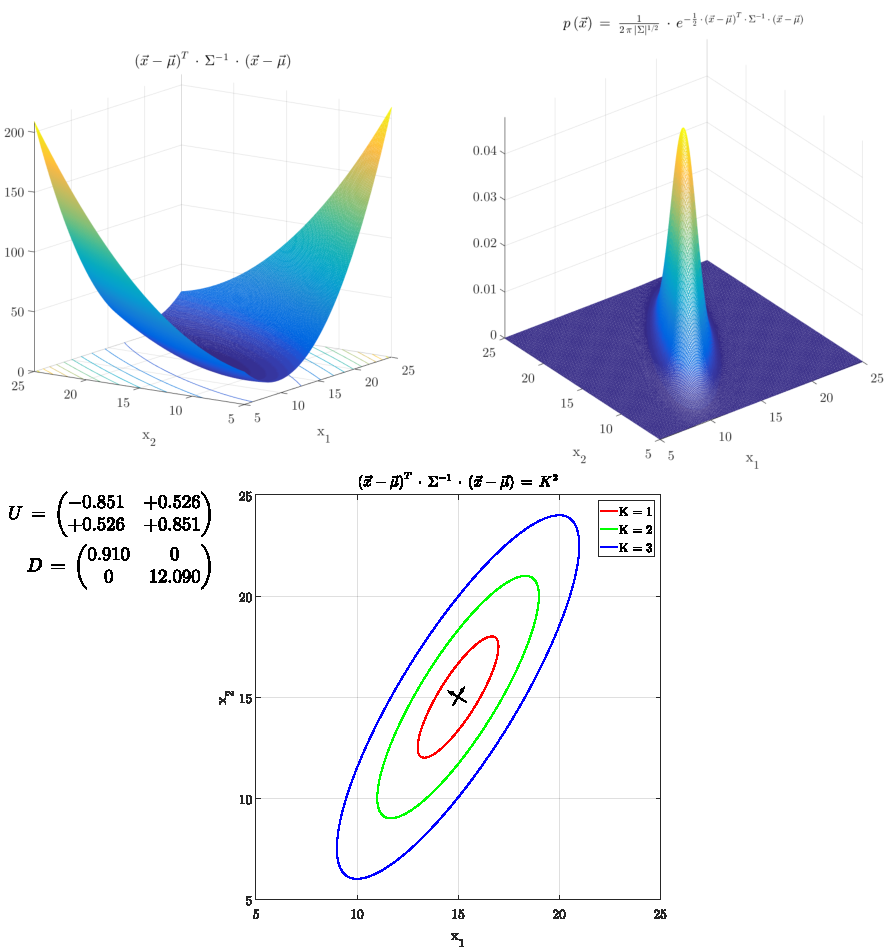
\includegraphics[scale=0.95]{../FIGURES/fig17}
\end{figure}

\newpage

\begin{align*}
\mu \, = \, \begin{pmatrix} 15 \\ 15 \end{pmatrix} ~ \Sigma \, = \, \begin{pmatrix} 
2^2 & -5\\
-5 & 3^2
\end{pmatrix} 
\end{align*}

\begin{figure}[H]
\centering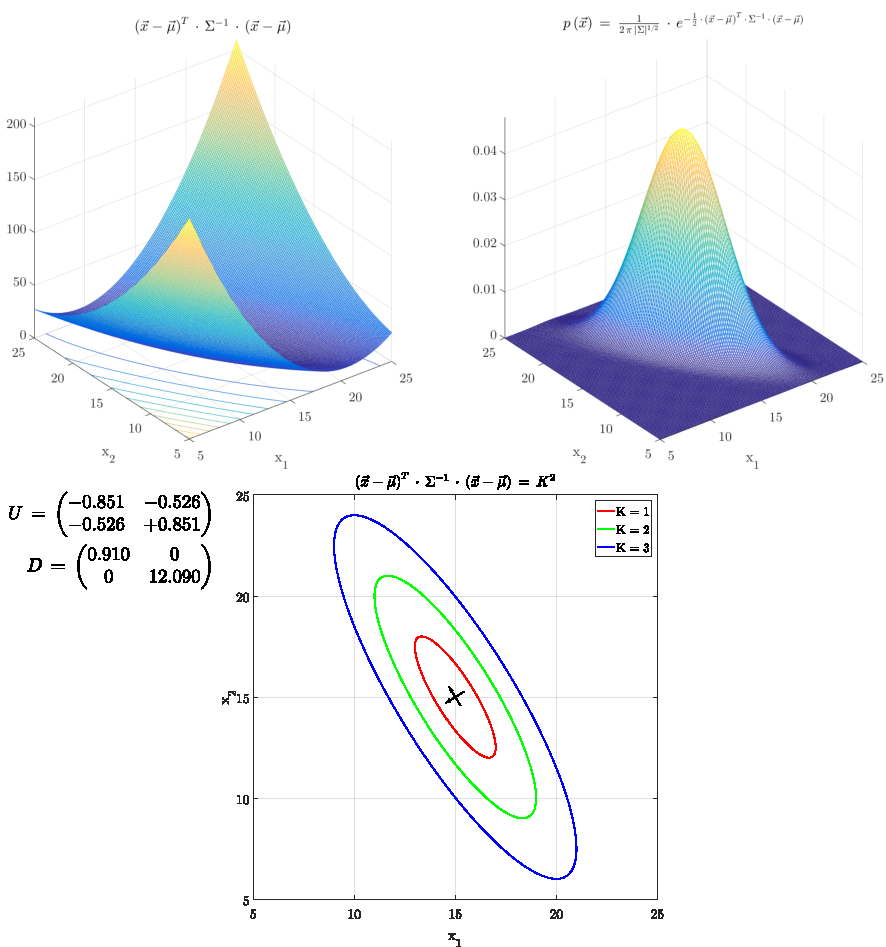
\includegraphics[scale=0.95]{../FIGURES/fig18}
\end{figure}

\newpage

\begin{align*}
\mu \, = \, \begin{pmatrix} 15 \\ 15 \end{pmatrix} ~ \Sigma \, = \, \begin{pmatrix} 
3^2 & 5\\
5 & 2^2
\end{pmatrix} 
\end{align*}

\begin{figure}[H]
\centering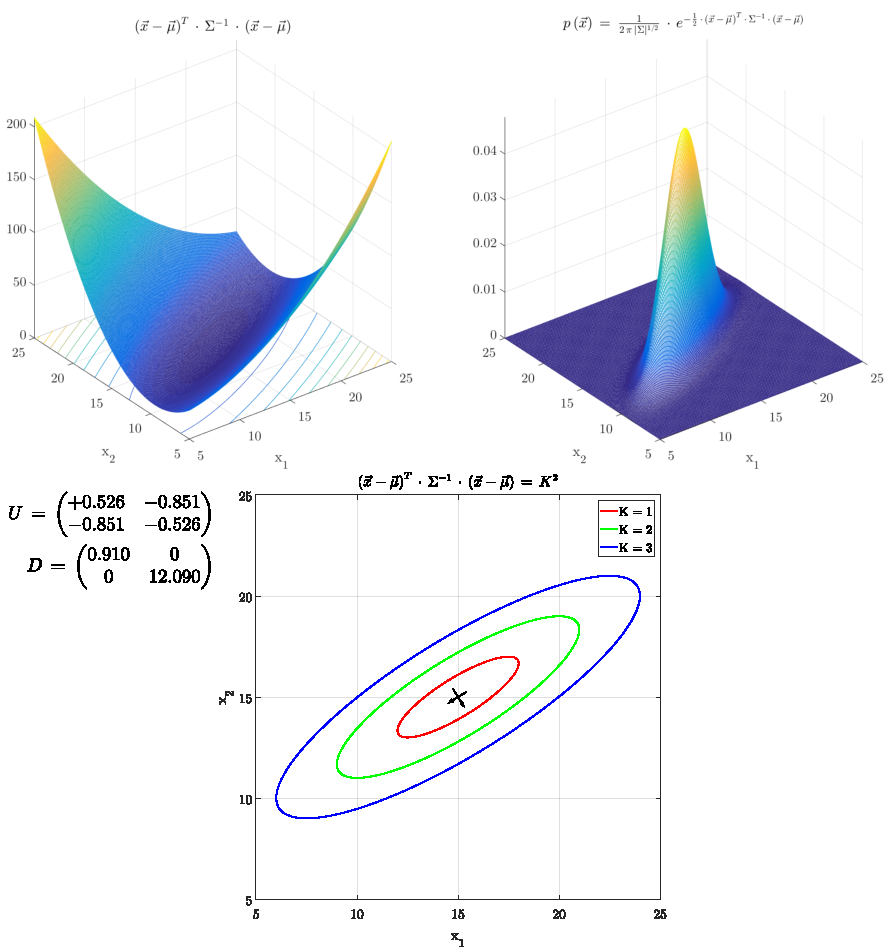
\includegraphics[scale=0.95]{../FIGURES/fig19}
\end{figure}

\newpage

\begin{align*}
\mu \, = \, \begin{pmatrix} 15 \\ 15 \end{pmatrix} ~ \Sigma \, = \, \begin{pmatrix} 
3^2 & -5\\
-5 & 2^2
\end{pmatrix} 
\end{align*}

\begin{figure}[H]
\centering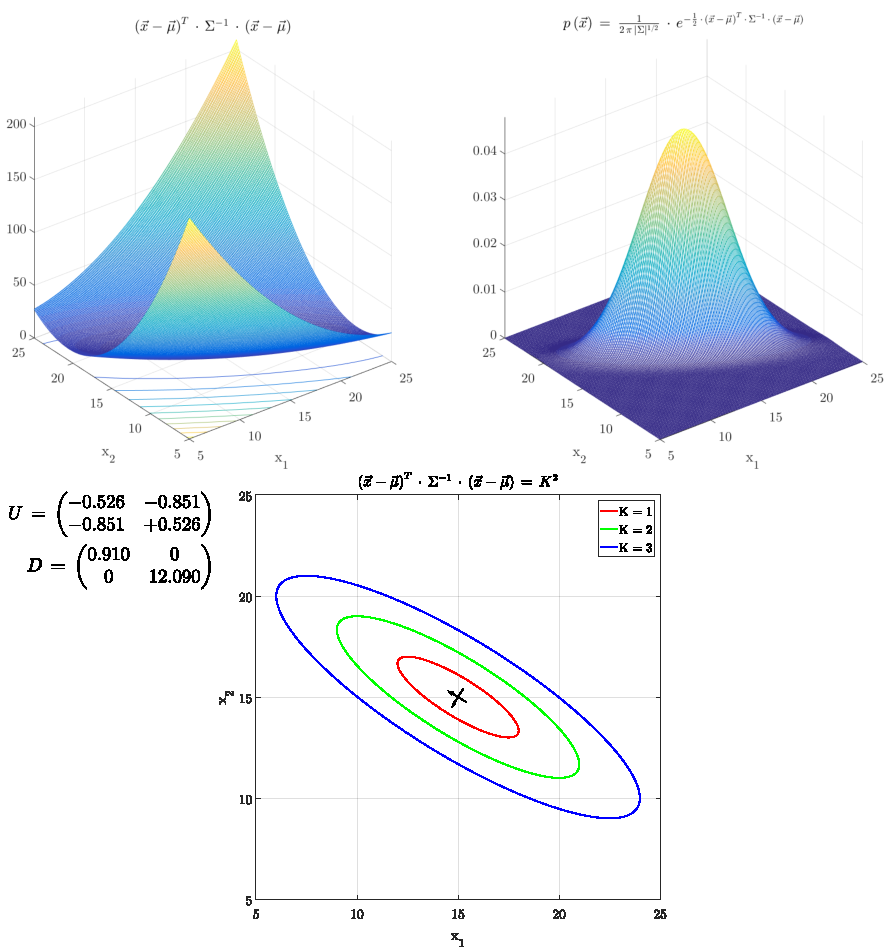
\includegraphics[scale=0.95]{../FIGURES/fig20}
\end{figure}

\newpage

If $\sigma_{x_1} \, = \, \sigma_{x_2}$

\begin{gather*}
\vec{u}_1 \, = \, \begin{pmatrix} +\,\frac{1}{\sqrt{2}}\\ +\,\frac{1}{\sqrt{2}} \end{pmatrix} \text{ or } \begin{pmatrix} -\,\frac{1}{\sqrt{2}}\\ -\,\frac{1}{\sqrt{2}} \end{pmatrix}\\
\vec{u}_2 \, = \, \begin{pmatrix} +\,\frac{1}{\sqrt{2}}\\ -\,\frac{1}{\sqrt{2}} \end{pmatrix} \text{ or } \begin{pmatrix} -\,\frac{1}{\sqrt{2}}\\ +\,\frac{1}{\sqrt{2}} \end{pmatrix}\\
\lambda_1 \, = \, \sigma_{x_1}^2\,\left(1\,+\,\rho\right)\,=\,\sigma_{x_1}^2\,+\,\sigma_{x_1x_2}\\
\lambda_2 \, = \, \sigma_{x_1}^2\,\left(1\,-\,\rho\right)\,=\,\sigma_{x_1}^2\,-\,\sigma_{x_1x_2}
\end{gather*}

Therefore, if $\sigma_{x_1x_2} \, > \, 0$, then the major axis of
the ellipse will be in the direction of the $45^{\circ}$ line and
the minor axis of the ellipse will be in the direction of the $135^{\circ} \left(45^{\circ} \, + \, 90^{\circ}\right)$
line.

Therefore, if $\sigma_{x_1x_2} \, < \, 0$, then the major axis of
the ellipse will be in the direction of the $135^{\circ}$ line and
the minor axis of the ellipse will be in the direction of the $45^{\circ} \left(135^{\circ} \, - \, 90^{\circ}\right)$
line.

\newpage

\begin{align*}
\mu \, = \, \begin{pmatrix} 15 \\ 15 \end{pmatrix} ~ \Sigma \, = \, \begin{pmatrix} 
3^2 & 5\\
5 & 3^2
\end{pmatrix} 
\end{align*}

\begin{figure}[H]
\centering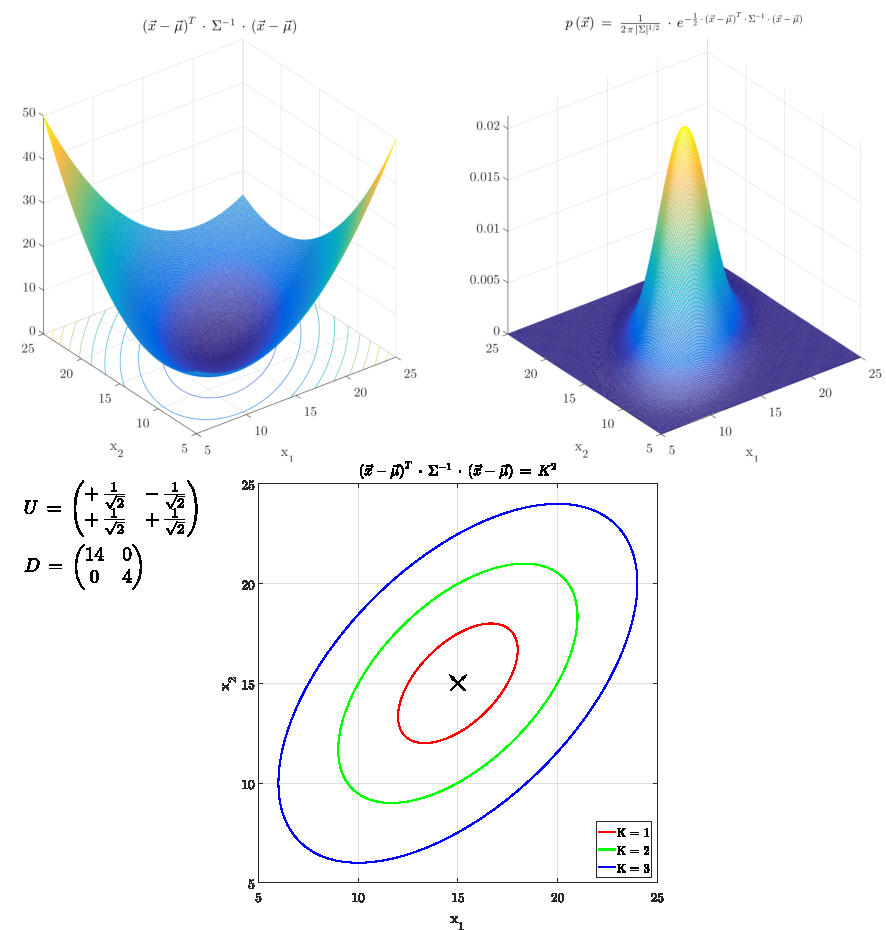
\includegraphics[scale=0.95]{../FIGURES/fig26}
\end{figure}

\newpage

\begin{align*}
\mu \, = \, \begin{pmatrix} 15 \\ 15 \end{pmatrix} ~ \Sigma \, = \, \begin{pmatrix} 
3^2 & -5\\
-5 & 3^2
\end{pmatrix} 
\end{align*}

\begin{figure}[H]
\centering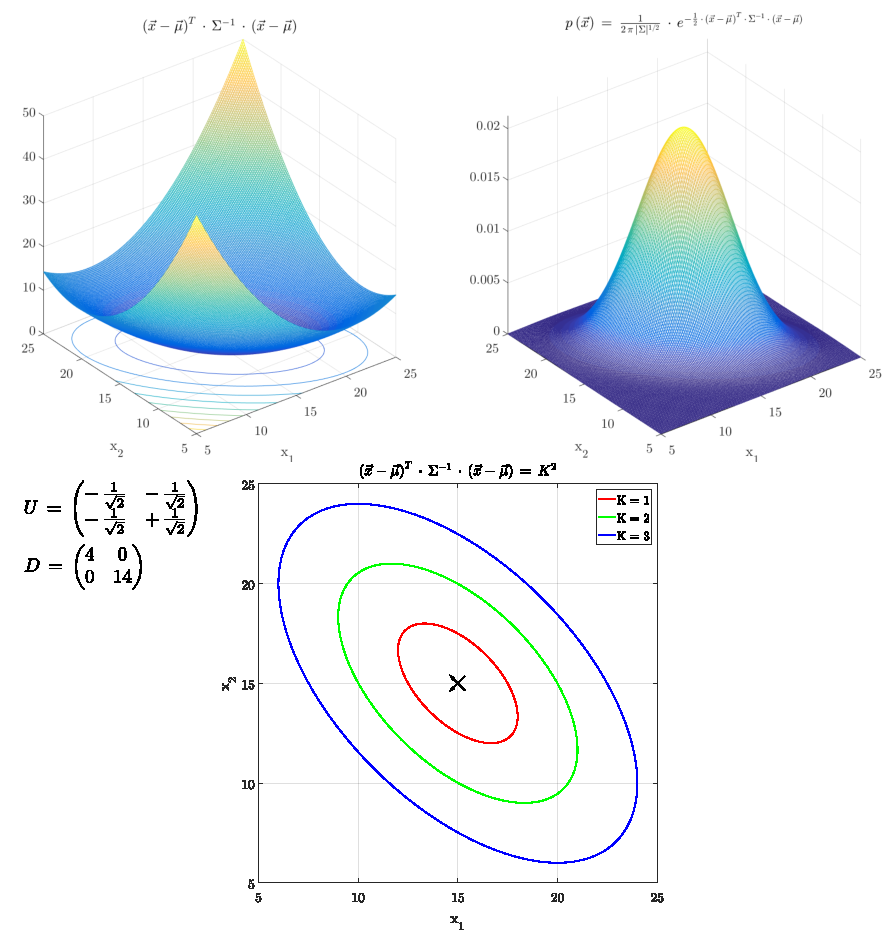
\includegraphics[scale=0.95]{../FIGURES/fig27}
\end{figure}

\newpage

Let's describe briefly how to plot a 2D ellipse given the directions
and lengths of its two principal axes. The directions of the ellipse's
two principal axes are given by the orthonormal eigenvectors $\vec{u}_1$
and $\vec{u}_2$. The length of the ellipse's two principal axes are
given by $2\,K\,\sqrt{\lambda_1}$ and $2\,K\,\sqrt{\lambda_2}$.

\begin{align*}
U \, = \, \begin{pmatrix}
u_{11} & u_{21}\\
u_{12} & u_{22}
\end{pmatrix} ~~~~~ D \, = \, \begin{pmatrix}
\lambda_1 & 0\\
0 & \lambda_2
\end{pmatrix}
\end{align*}
\begin{align*}
\begin{pmatrix}
x_1 & y_1\\
\vdots & \vdots\\
x_j & y_j\\
\vdots & \vdots\\
x_M & y_M\\
\end{pmatrix}
\, &= \, K \, \begin{pmatrix}
\cos\left(\theta_1\right) & \sin\left(\theta_1\right)\\
\vdots & \vdots\\
\cos\left(\theta_j\right) & \sin\left(\theta_j\right)\\
\vdots & \vdots\\
\cos\left(\theta_M\right) & \sin\left(\theta_M\right)\\
\end{pmatrix} \, \cdot \, \begin{pmatrix}
\sqrt{\lambda_1} & 0\\
0 & \sqrt{\lambda_2}
\end{pmatrix} \, \cdot \, \begin{pmatrix}
u_{11} & u_{12}\\
u_{21} & u_{22}
\end{pmatrix} \,=\\
&= \, K \, \begin{pmatrix}
\cos\left(\theta_1\right) & \sin\left(\theta_1\right)\\
\vdots & \vdots\\
\cos\left(\theta_j\right) & \sin\left(\theta_j\right)\\
\vdots & \vdots\\
\cos\left(\theta_M\right) & \sin\left(\theta_M\right)\\
\end{pmatrix} \, \cdot \, \begin{pmatrix}
\sqrt{\lambda_1}\,u_{11} & \sqrt{\lambda_1}\,u_{12}\\
\sqrt{\lambda_2}\,u_{21} & \sqrt{\lambda_2}\,u_{22}
\end{pmatrix} \, =\\
&= \, K \, \begin{pmatrix}
\sqrt{\lambda_1}\,u_{11}\,\cos\left(\theta_1\right) \, + \,  \sqrt{\lambda_2}\,u_{21}\,\sin\left(\theta_1\right) &  \sqrt{\lambda_1}\,u_{12}\,\cos\left(\theta_1\right) \, + \,  \sqrt{\lambda_2}\,u_{22}\,\sin\left(\theta_1\right)\\
\vdots & \vdots\\
\sqrt{\lambda_1}\,u_{11}\,\cos\left(\theta_j\right) \, + \,  \sqrt{\lambda_2}\,u_{21}\,\sin\left(\theta_j\right) &  \sqrt{\lambda_1}\,u_{12}\,\cos\left(\theta_j\right) \, + \,  \sqrt{\lambda_2}\,u_{22}\,\sin\left(\theta_j\right)\\
\vdots & \vdots\\
\sqrt{\lambda_1}\,u_{11}\,\cos\left(\theta_M\right) \, + \,  \sqrt{\lambda_2}\,u_{21}\,\sin\left(\theta_M\right) &  \sqrt{\lambda_1}\,u_{12}\,\cos\left(\theta_M\right) \, + \,  \sqrt{\lambda_2}\,u_{22}\,\sin\left(\theta_M\right)
\end{pmatrix} 
\end{align*}
\begin{gather*}
\theta_j \, = \, \frac{360}{M}\,j\\j \,=\, 0,\, \ldots,\, M\,-\,1\\
\begin{pmatrix} \text{M is the desired number of points to draw} \end{pmatrix}
\end{gather*}

Now, I'm going to describe one particular case that occurs when $\sigma_{x_1x_2} \, = \,0$,
which it's the same as saying $\rho \, = \, 0$.

When \begin{gather*}
\sigma_{x_1x_2} \, = \, \rho \, \sigma_{x_1} \, \sigma_{x_2} \, \neq \, 0\\
\begin{pmatrix} -1 \, < \, \rho \, < \, 1 \end{pmatrix}
\end{gather*} the variables $x_1$ and $x_2$ are correlated. 

When 

\begin{gather*}
\sigma_{x_1x_2} \, = \, \rho \, \sigma_{x_1} \, \sigma_{x_2} \, = \, 0\\
\begin{pmatrix} \rho \, = \, 0 \end{pmatrix}
\end{gather*} the variables $x_1$ and $x_2$ are incorrelated. Now, one interesting
result stands that if the joint distribution among $N$ random variables
is Gaussian, then the marginal distribution of each random variable
is also Gaussian, even the conditional distributions are Gaussian.
The other way around is not true. If you have $N$ random variables,
each of those distributed following a Gaussian PDF, then the random
vector doesn't have to be distributed following a Gaussian PDF \footnote{Not 100\% sure about this last fact. If you ever need this result,
check it out firstly.}

So because the joint distribution between the random variables $x_1$
and $x_2$ is Gaussian, then the random variables $x_1$ and $x_2$
are also distributed accordingly to Gaussian PDFs. For random variables
distributed accordingly to Gaussian distributions incorrelation implies
independency.

Every computation is easier when $\sigma_{x_1x_2} \, = \, 0$.

\begin{gather*}
\Sigma \, = \, \begin{pmatrix} 
\sigma_{x_1}^2 & 0 & \ldots & 0 & \ldots & 0\\
0 & \sigma_{x_2}^2 & \ldots & 0 & \ldots & 0\\
\vdots & \vdots & \ddots & \vdots & \vdots & \vdots\\
0 & 0 & \ldots & \sigma_{x_j}^2 & \ldots & 0\\
\vdots & \vdots & \vdots & \vdots & \ddots & \vdots\\
0 & 0 & \ldots & 0 & \ldots & \sigma_{x_N}^2\\
\end{pmatrix} \, = \, \sum_{j \, = \, 1}^N \lambda_j\,\vec{e}_j\,\vec{e}_j^{\,T}\\\\
\vec{e}_j \, = \, \begin{pmatrix} 0\\ 0\\ \vdots\\ 1\\ \vdots\\ 0 \end{pmatrix} \begin{matrix} \textcolor{white}{0}\\ \textcolor{white}{0}\\ \textcolor{white}{\vdots}\\ \longleftarrow ~ j-th  \text{ position}\\ \textcolor{white}{\vdots}\\ \textcolor{white}{0}\end{matrix}\\\\
\lambda_j \, = \, \sigma_{x_j}^2
\end{gather*}

\begin{gather*}
\Sigma^{-1} \, = \, \sum_{j \, = \, 1}^N \frac{1}{\lambda_j}\,\vec{e}_j\,\vec{e}_j^{\,T} \, = \, \begin{pmatrix} 
1/\sigma_{x_1}^2 & 0 & \ldots & 0 & \ldots & 0\\
0 & 1/\sigma_{x_2}^2 & \ldots & 0 & \ldots & 0\\
\vdots & \vdots & \ddots & \vdots & \vdots & \vdots\\
0 & 0 & \ldots & 1/\sigma_{x_j}^2 & \ldots & 0\\
\vdots & \vdots & \vdots & \vdots & \ddots & \vdots\\
0 & 0 & \ldots & 0 & \ldots & 1/\sigma_{x_N}^2\\
\end{pmatrix}
\end{gather*}

Particularizing for the 2D Gaussian:

\begin{align*}
\Sigma \, &= \, 
\begin{pmatrix} 
\sigma_{x_1}^2 & 0\\
0 & \sigma_{x_2}^2
\end{pmatrix}\\\\
\Sigma^{-1} \, &= \, 
\begin{pmatrix} 
\frac{1}{\sigma_{x_1}^2} & 0\\
0 & \frac{1}{\sigma_{x_2}^2}
\end{pmatrix}
\end{align*}

\begin{gather*}
\vec{e}_1 \, = \, \begin{pmatrix} 1\\ 0\end{pmatrix} ~~ \vec{e}_2 \, = \, \begin{pmatrix} 0\\ 1\end{pmatrix}\\\\
\lambda_1 \, = \, \sigma_{x_1}^2 ~~ \lambda_2 \, = \, \sigma_{x_2}^2
\end{gather*}

\begin{align*}
\left\langle \left(\vec{x} \, - \, \vec{\mu}\right), ~ \Sigma^{-1} \, \cdot \, \left(\vec{x} \, - \, \vec{\mu}\right) \right\rangle \, &= \, \left(\vec{x} \, - \, \vec{\mu}\right)^T \, \cdot \, \Sigma^{-1} \, \cdot \, \left(\vec{x} \, - \, \vec{\mu}\right) \, =\\
&= \, \begin{pmatrix}x_1 \, - \, \mu_1, x_2 \, - \, \mu_2 \end{pmatrix} \, \cdot \,
\begin{pmatrix} 
\frac{1}{\sigma_{x_1}^2} & 0\\
0 & \frac{1}{\sigma_{x_2}^2}
\end{pmatrix} \, \cdot \, \begin{pmatrix}x_1 \, - \, \mu_1\\ x_2 \, - \, \mu_2 \end{pmatrix} \, =\\
&= \, \frac{\left(x_1 \, - \, \mu_1\right)^2}{\sigma_{x_1}^2} \, + \, \frac{\left(x_2 \, - \, \mu_2\right)^2}{\sigma_{x_2}^2}\\
&= \, \frac{e_{11}^2}{\lambda_1}\,\cdot\,\left(x_1 \, - \, \mu_1\right)^2 \, + \, \frac{e_{22}^2}{\lambda_2}\,\cdot\,\left(x_2 \, - \, \mu_2\right)^2
\end{align*}

The following expression corresponds to an ellipse centered at the
vector $\vec{\mu}$, with the directions of its principal axes defined
by the orthonormal eigenvectors $\vec{e}_1$ and $\vec{e}_2$, i.e,
they are parallels to the x-axis and y-axis, and with the length of
its principal axes defined by $K\sigma_{x_1}$.

\begin{align*}
\left\langle \left(\vec{x} \, - \, \vec{\mu}\right), ~ \Sigma^{-1} \, \cdot \, \left(\vec{x} \, - \, \vec{\mu}\right) \right\rangle \, &= \, \left(\vec{x} \, - \, \vec{\mu}\right)^T \, \cdot \, \Sigma^{-1} \, \cdot \, \left(\vec{x} \, - \, \vec{\mu}\right) \, =\\
&= \, \frac{\left(x_1 \, - \, \mu_1\right)^2}{\sigma_{x_1}^2} \, + \, \frac{\left(x_2 \, - \, \mu_2\right)^2}{\sigma_{x_2}^2} \, = \, K^2
\end{align*}

\begin{align*}
\left(\frac{x_1 \, - \, \mu_1}{K\,\sigma_{x_1}}\right)^2 \, + \, \left(\frac{x_2 \, - \, \mu_2}{K\,\sigma_{x_2}}\right)^2 \, = \, 1
\end{align*}

\newpage

\begin{align*}
\mu \, = \, \begin{pmatrix} 15 \\ 15 \end{pmatrix} ~ \Sigma \, = \, \begin{pmatrix} 
1^2 & 0\\
0 & 3^2
\end{pmatrix} 
\end{align*}

\begin{figure}[H]
\centering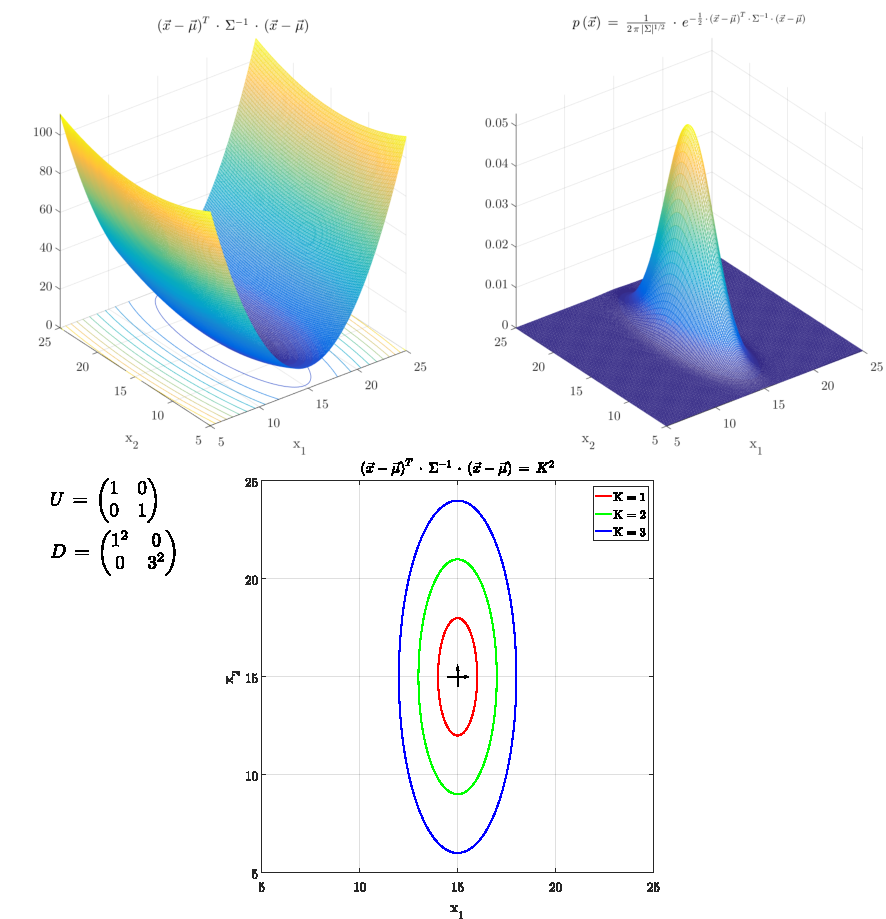
\includegraphics[scale=0.95]{../FIGURES/fig35}
\end{figure}

\newpage

\begin{align*}
\mu \, = \, \begin{pmatrix} 15 \\ 15 \end{pmatrix} ~ \Sigma \, = \, \begin{pmatrix} 
3^2 & 0\\
0 & 1^2
\end{pmatrix} 
\end{align*}

\begin{figure}[H]
\centering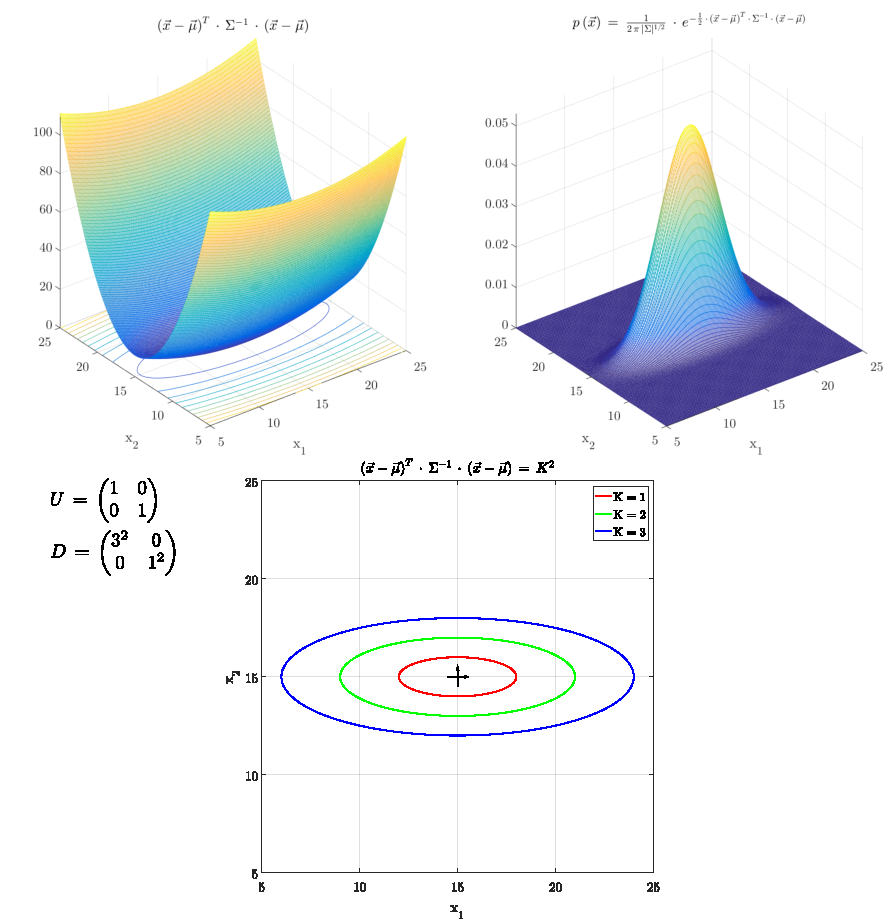
\includegraphics[scale=0.95]{../FIGURES/fig36}
\end{figure}

\newpage

\begin{align*}
\mu \, = \, \begin{pmatrix} 15 \\ 15 \end{pmatrix} ~ \Sigma \, = \, \begin{pmatrix} 
3^2 & 0\\
0 & 3^2
\end{pmatrix} 
\end{align*}

\begin{figure}[H]
\centering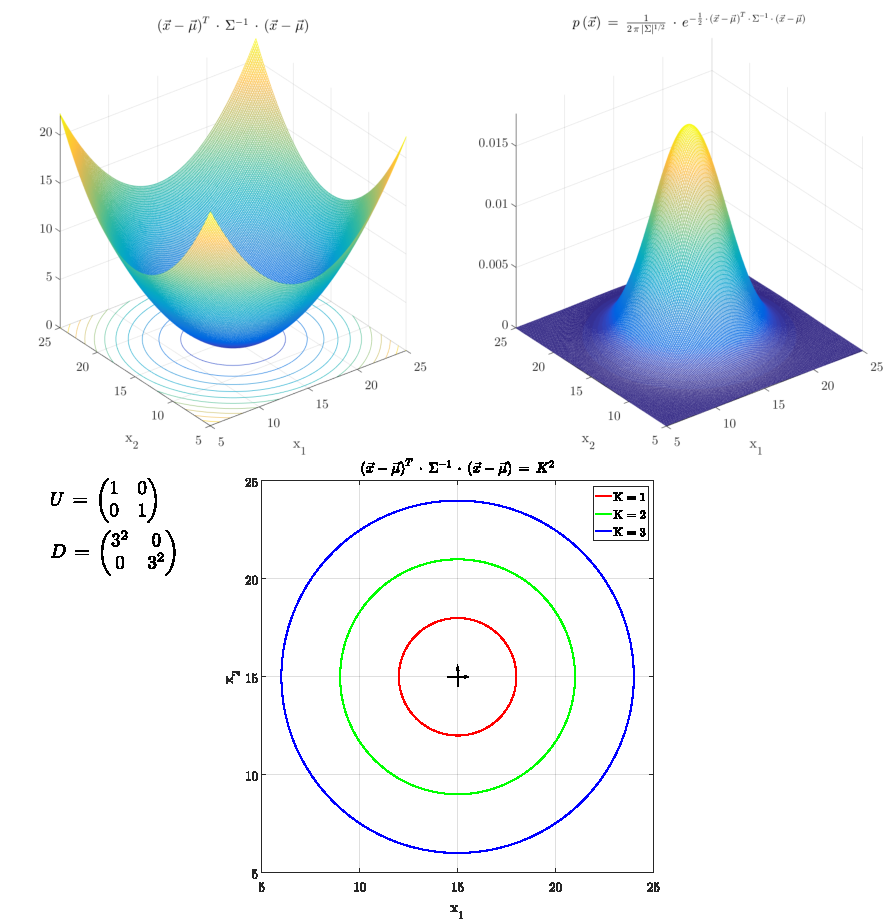
\includegraphics[scale=0.95]{../FIGURES/fig37}
\end{figure}

So, as we can see, when $\sigma_{x_1x_2} \, = \, 0$:
\begin{itemize}
\item If $\sigma_{x_1} \, > \, \sigma_{x_2}$ then the ellipse has its major
axis along the x-axis.
\item If $\sigma_{x_2} \, > \, \sigma_{x_1}$ then the ellipse has its major
axis along the y-axis.
\item If $\sigma_{x_1} \, = \, \sigma_{x_2}$ then the ellipse converts
into a circumference, and its radius is equal $r \, = \, K\sigma_{x_1} \, = \, K\sigma_{x_2}$.
\end{itemize}
Exercise:

Let's consider a brief exercise. Let's suppose that we are partially
given a Gaussian joint distribution between the random variable $x_1$
and the random variable $x_2$.

\begin{gather*}
\vec{x} \, = \,
\begin{pmatrix}
x_1\\
x_2
\end{pmatrix} ~~~~~ p\left(\vec{x}\right) \, = \, \mathcal{N}\left(\vec{\mu}, \Sigma\right) ~~~~~ \vec{\mu} \, = \, \begin{pmatrix}
\mu_1\\
\mu_2
\end{pmatrix} ~~~~~ \Sigma \, = \, \begin{pmatrix} \sigma^2 & ?\\ ? & \sigma^2 \end{pmatrix}
\end{gather*}

With the given partial Gaussian joint distribution let's try to associate
it with one of the pictures below.

\begin{figure}[H]
\centering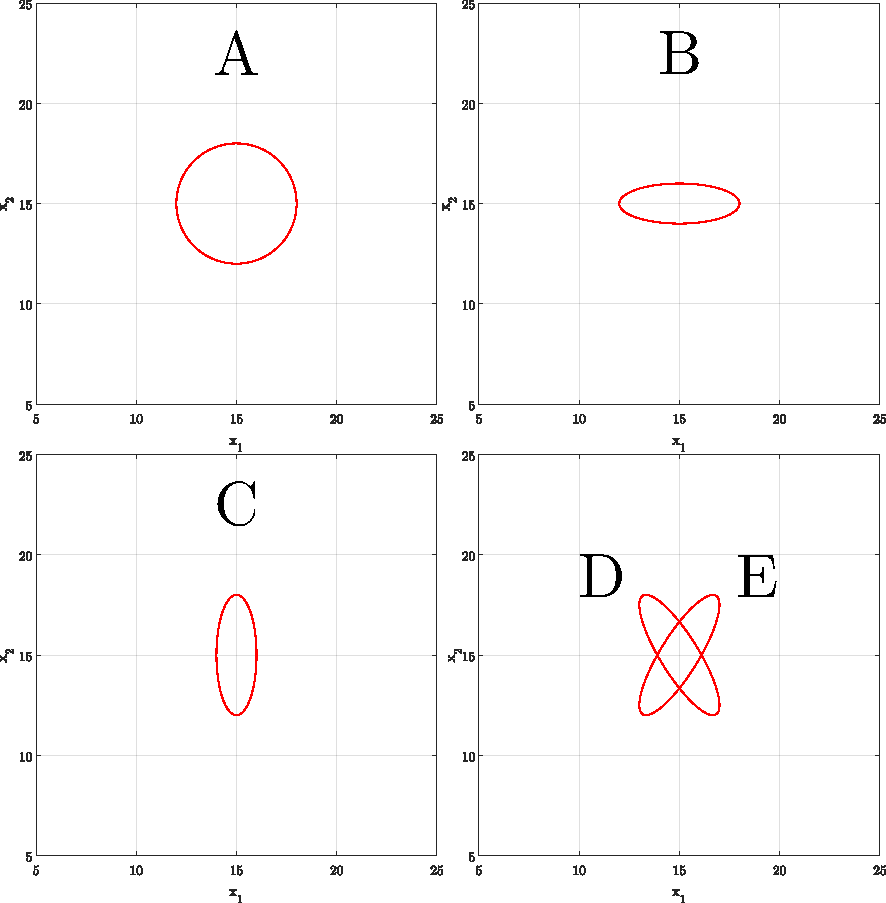
\includegraphics[scale=0.95]{../FIGURES/fig39}
\end{figure}

First thing $\sigma_{x_1}^2 \, = \, \sigma_{x_2}^2 \, = \, \sigma^2$. 

If $\sigma_{x_1x_2} \, = \, 0$, then we would have a circumference.
So, figure A.

If $\sigma_{x_1x_2} \, \neq \, 0$, then we would have an ellipse.
If $\sigma_{x_1x_2} \, > \, 0$, then the major axis of the ellipse
will be in the direction of the $45^{\circ}$ line and the minor axis
of the ellipse will be in the direction of the $135^{\circ} \left(45^{\circ} \, + \, 90^{\circ}\right)$
line. So, figure E.

If $\sigma_{x_1x_2} \, < \, 0$, then the major axis of the ellipse
will be in the direction of the $135^{\circ}$ line and the minor
axis of the ellipse will be in the direction of the $45^{\circ} \left(135^{\circ} \, - \, 90^{\circ}\right)$
line. So, figure D.

We would have the figure B when $\sigma_{x_1}^2 \, > \, \sigma_{x_2}^2$
and $\sigma_{x_1x_2} \, = \, 0$.

We would have the figure C when $\sigma_{x_1}^2 \, < \, \sigma_{x_2}^2$
and $\sigma_{x_1x_2} \, = \, 0$.

Therefore, since we have $\sigma_{x_1}^2 \, = \, \sigma_{x_2}^2 \, = \, \sigma^2$
we can't have either figure B or figure C.\\
\\
\begin{center}
\textbf{EXERCISE}
\par\end{center}

The lever arm is fixed to the wall at the point $A$. The lever arm
can rotate around the point A. The motor moves the point $P$ a distance
$x$. First, calculate the relation between the random variable $y$
and the random variable $x$. Calculate the eigenvalues and the eigenvectors
of the covariance matrix $\Sigma$ that results from the relation
between the random variables $x$ and $y$.

\begin{figure}[H]
\centering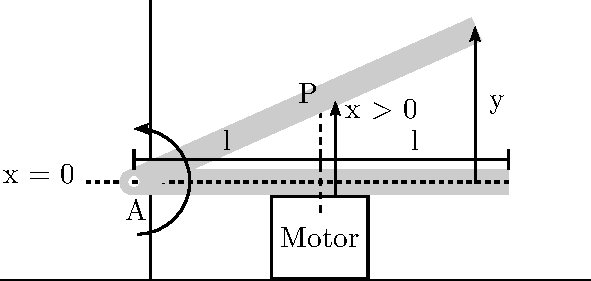
\includegraphics[scale=0.95]{../FIGURES/fig41}
\end{figure}

\begin{figure}[H]
\centering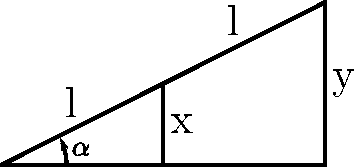
\includegraphics[scale=0.95]{../FIGURES/fig42}
\end{figure}

The free extreme of the lever arm moves a distance:

gather\begin{gather*}
\sin\left(\alpha\right) \, = \, \frac{x}{l}\\
y \, = \, 2l \, \sin\left(\alpha\right) \, = \, 2l \, \frac{x}{l} \, = \, 2x
\end{gather*}

We are told that the error in the motor motion, i.e, the error in
the $x$ distance is:

\begin{align*}
e_x \, &= \, \mathcal{N}\left(\mu,\, \sigma_x^2\right)\\
\mu \, &= \, 0
\end{align*}

The distance $y$ only depends on the motor, so, because the motor
has an inherent error $e_x$ that is distributed according to a Gaussian
distribution, the error in the motion in the free extreme of the lever
arm also follows a Gaussian distribution. Let's suppose that the motor
moves a distance $x$ with some error:

\begin{align*}
x' \, &= \, x \, + \, e_x\\
y' \, &= \, y \, + \, e_y \, = \, 2x' \, = \, 2\left(x \, + \, e_x\right) \, = \, 2x \, + \, 2e_x\\
y \, &= \, 2x\\
e_y \, &= \, 2e_x
\end{align*}

\begin{align*}
\mu_x \, &\triangleq \, E\left(e_x\right) \, = \, 0\\
\sigma_x^2 \, &\triangleq \, E\left(\left(e_x \, - \, E\left(e_x\right)\right)^2\right) \, = \, E\left(e_x^2\right)\\
\mu_y \, &\triangleq \, E\left(e_y\right) \, = \, E\left(2e_x\right) \, = \, 2E\left(e_x\right) \, = \, 0\\
\sigma_y^2 \, &\triangleq \, E\left(\left(e_y \, - \, E\left(e_y\right)\right)^2\right) \, = \, E\left(e_y^2\right) \, = \, E\left(4e_x^2\right) \, = \, 4E\left(e_x^2\right) \, = \, 4\sigma_x^2
\end{align*}

\begin{align*}
e_y \, = \, \mathcal{N}\left(0,\, 4\sigma_x^2\right)
\end{align*}

\begin{align*}
\vec{e} \, = \, \begin{pmatrix}e_x \\ e_y  \end{pmatrix}
\end{align*}

\begin{align*}
\Sigma \, &= \, E\left(\left(\vec{e} \, - \, E\left(\vec{e}\right)\right)\,\left(\vec{e} \, - \, E\left(\vec{e}\right)\right)^T\right) \, = \, E\left(\vec{e} \, \cdot \, \vec{e}^{\,T}\right) \, = \, E\begin{pmatrix} \begin{pmatrix}e_x\\ e_y \end{pmatrix} \, \cdot \, \begin{pmatrix}e_x & e_y \end{pmatrix} \end{pmatrix} \, = \, E\begin{pmatrix} \begin{pmatrix} e_x^2 & e_xe_y\\ e_xe_y & e_y^2 \end{pmatrix}\end{pmatrix} \,=\\
&= \, E\begin{pmatrix}\begin{pmatrix}e_x^2 & 2e_x^2\\ 2e_x^2 & 4e_x^2 \end{pmatrix}\end{pmatrix} \, = \, \begin{pmatrix}\sigma_x^2 & 2\sigma_x^2\\ 2\sigma_x^2 & 4\sigma_x^2 \end{pmatrix} \, = \, \sigma_x^2 \, \begin{pmatrix}1 & 2\\ 2 & 4 \end{pmatrix}
\end{align*}

\begin{align*}
\sigma_{x_1} \,&=\, \sigma_x\\
\sigma_{x_2} \,&=\, 2\,\sigma_x\\
\sigma_{x_1x_2} \,&= \, 2\,\sigma_x^2\\
\rho \,&=\, \frac{\sigma_{x_1x_2}}{\sigma_{x_1}\,\sigma_{x_2}} \,=\, \frac{2\,\sigma_x^2}{\sigma_x \, 2\,\sigma_x} \,=\, 1
\end{align*}

Obviously, $\rho \, = \, 1$ because the relation between the random
variables $x$ and $y$ is linear.

Calculate the eigenvalues and eigenvectors of the covariance matrix
$\Sigma$.

\begin{align*}
\begin{vmatrix}
\Sigma \, - \, \lambda_j\,I
\end{vmatrix} \, &= \, \begin{vmatrix}
\sigma_x^2 \, \begin{pmatrix}1 & 2\\ 2 & 4 \end{pmatrix} \, - \, \begin{pmatrix}\lambda_j & 0\\ 0 & \lambda_j \end{pmatrix}
\end{vmatrix} \, = \, \begin{vmatrix} \begin{pmatrix}\sigma_x^2 \, - \, \lambda_j & 2\sigma_x^2\\ 2\sigma_x^2 & 4\sigma_x^2 \, - \, \lambda_j \end{pmatrix}\end{vmatrix} \, =\\
&= \, \left(\sigma_x^2 \, - \, \lambda_j\right)\left(4\,\sigma_x^2 \, - \, \lambda_j\right) \, - \, 4\,\sigma_x^2 \, = \, -\,\lambda_j\,\sigma_x^2 \, - \, 4\,\sigma_x^2\,\lambda_j \, + \, \lambda_j^2 \,=\\
&= \, \lambda_j^2 \, - \, 5\,\sigma_x^2\lambda_j \, = \, \lambda_j\,\left(\lambda_j \, - \, 5\,\sigma_x^2\right) \, = \, 0
\end{align*}

\begin{align*}
\lambda_1 \, &= \, 0\\
\lambda_2 \, &= \, 5\sigma_x^2\\
\end{align*}

\begin{align*}
\begin{pmatrix}
\Sigma \, - \, \lambda_1\,I 
\end{pmatrix} \, \cdot \, \vec{u}_1 \, = \, \begin{pmatrix}\sigma_x^2 \, \begin{pmatrix}1 & 2\\ 2 & 4 \end{pmatrix} \, - \, \begin{pmatrix}\lambda_1 & 0\\ 0 & \lambda_1\end{pmatrix}\end{pmatrix} \,\cdot\, \begin{pmatrix}u_{11}\\u_{12} \end{pmatrix} \, = \, \sigma_x^2 \, \begin{pmatrix}1 & 2\\ 2 & 4 \end{pmatrix} \,\cdot\, \begin{pmatrix}u_{11}\\u_{12} \end{pmatrix} \, = \, \begin{pmatrix}0\\0\end{pmatrix}
\end{align*}

\begin{align*}
\sigma_x^2\,u_{11} \, + \, 2\,\sigma_x^2\,u_{12} \, &= \, 0\\
2\,\sigma_x^2\,u_{11} \, + \, 4\,\sigma_x^2\,u_{12} \, &= \, 0 ~ \longrightarrow ~ \sigma_x^2\,u_{11} \, + \, 2\,\sigma_x^2\,u_{12} \, = \, 0
\end{align*}

\lyxaddress{\begin{align*}
u_{11} \, = \, -\,\frac{2\,\sigma_x^2}{\sigma_x^2}\,u_{12} \, = \, -2\,u_{12}
\end{align*}}

We choose:

\lyxaddress{\begin{gather*}
u_{12} \, = \, 1 ~ \longrightarrow ~ u_{11} \, = \, -\,2\\
\vec{u}_1 \, = \, \begin{pmatrix} -\,2\\+\,1\end{pmatrix} 
\end{gather*}}

Now, the vector $\vec{u}_1$ is normalized:

\begin{gather*}
\lVert \vec{u}_1 \rVert \, = \, \sqrt{\langle \vec{u}_1,\, \vec{u}_1 \rangle} \, = \, \sqrt{\vec{u}_1^{\,T} \, \cdot \, \vec{u}_1} \, = \, \sqrt{u_{11}^2 \, + \, u_{12}^2} \, = \, \sqrt{\left(-\,2\right)^2 \,+\, 1^2} \, = \, \sqrt{5}\\
\vec{u}_1 \, = \, \begin{pmatrix} \frac{u_{11}}{\lVert \vec{u}_1 \rVert} \\ \frac{u_{12}}{\lVert \vec{u}_1 \rVert} \end{pmatrix} \,=\, \begin{pmatrix} -\,\frac{2}{\sqrt{5}}\\ +\,\frac{1}{\sqrt{5}}\end{pmatrix}
\end{gather*}

\begin{align*}
\begin{pmatrix}
\Sigma \, - \, \lambda_2\,I 
\end{pmatrix} \, \cdot \, \vec{u}_2 \, &= \, \begin{pmatrix}\sigma_x^2 \, \begin{pmatrix}1 & 2\\ 2 & 4 \end{pmatrix} \, - \, \begin{pmatrix}\lambda_2 & 0\\ 0 & \lambda_2\end{pmatrix}\end{pmatrix} \,\cdot\, \begin{pmatrix}u_{21}\\u_{22} \end{pmatrix} \, = \, \begin{pmatrix} \sigma_x^2 \, \begin{pmatrix}1 & 2\\ 2 & 4 \end{pmatrix} \, - \, 5\,\sigma_x^2\begin{pmatrix}1 & 0\\ 0 & 1\end{pmatrix}\end{pmatrix} \,\cdot\, \begin{pmatrix}u_{21}\\u_{22} \end{pmatrix} \, =\\ 
&= \, \begin{pmatrix}-4\,\sigma_x^2 & 2\,\sigma_x^2\\ 2\,\sigma_x^2 & -\,\sigma_x^2 \end{pmatrix} \,\cdot\, \begin{pmatrix}u_{21}\\u_{22} \end{pmatrix}  = \, \begin{pmatrix}0\\0\end{pmatrix}
\end{align*}

\begin{align*}
-4\,\sigma_x^2\,u_{21} \, + \, 2\,\sigma_x^2\,u_{22} \, &= \, 0 ~ \longrightarrow ~ 2\,\sigma_x^2\,u_{21} \, - \, \sigma_x^2\,u_{22} \, = \, 0\\
2\,\sigma_x^2\,u_{21} \, - \, \sigma_x^2\,u_{22} \, &= \, 0
\end{align*}

\lyxaddress{\begin{align*}
u_{21} \, = \, \frac{\sigma_x^2}{2\,\sigma_x^2}\,u_{22} \, = \, \frac{1}{2}\,u_{22}
\end{align*}}

We choose:

\lyxaddress{\begin{gather*}
u_{22} \, = \, 2 ~ \longrightarrow ~ u_{21} \, = \, 1\\
\vec{u}_2 \, = \, \begin{pmatrix} +\,1\\+\,2\end{pmatrix} 
\end{gather*}}

Now, the vector $\vec{u}_2$ is normalized:

\begin{gather*}
\lVert \vec{u}_2 \rVert \, = \, \sqrt{\langle \vec{u}_2,\, \vec{u}_2 \rangle} \, = \, \sqrt{\vec{u}_2^{\,T} \, \cdot \, \vec{u}_2} \, = \, \sqrt{u_{21}^2 \, + \, u_{22}^2} \, = \, \sqrt{1^2 \,+\, 2^2} \, = \, \sqrt{5}\\
\vec{u}_2 \, = \, \begin{pmatrix} \frac{u_{21}}{\lVert \vec{u}_2\rVert} \\ \frac{u_{22}}{\lVert \vec{u}_2 \rVert} \end{pmatrix} \,=\, \begin{pmatrix} +\,\frac{1}{\sqrt{5}}\\ +\,\frac{2}{\sqrt{5}}\end{pmatrix}
\end{gather*}

\begin{align*}
\vec{u} \, = \, \begin{pmatrix} \mu_1\\ \mu_2\end{pmatrix} \, = \, \begin{pmatrix}0\\0\end{pmatrix}
\end{align*}

\begin{align*}
\Sigma \,=\, \sigma_x^2\,\begin{pmatrix}1 & 2\\ 2 & 4\end{pmatrix} \, &= \, \begin{pmatrix}u_{11} & u_{21}\\ u_{12} & u_{22}\end{pmatrix} \,\cdot\, \begin{pmatrix}\lambda_1 & 0\\ 0 & \lambda_2\end{pmatrix} \,\cdot\, \begin{pmatrix}u_{11} & u_{12}\\ u_{21} & u_{22}\end{pmatrix} \,=\\
&=\, \begin{pmatrix}-\,\frac{2}{\sqrt{5}} & +\,\frac{1}{\sqrt{5}}\\ +\,\frac{1}{\sqrt{5}} & +\,\frac{2}{\sqrt{5}}\end{pmatrix} \,\cdot\, \begin{pmatrix}0 & 0\\ 0 & 5\,\sigma_x^2\end{pmatrix} \,\cdot\, \begin{pmatrix}-\,\frac{2}{\sqrt{5}} & +\,\frac{1}{\sqrt{5}}\\ +\,\frac{1}{\sqrt{5}} & +\,\frac{2}{\sqrt{5}}\end{pmatrix}
\end{align*}

Let's plot the ellipse associated to the covariance matrix $\Sigma$
when $\sigma_x \, = \, 1$.

\begin{align*}
\Sigma \,=\, \begin{pmatrix}1 & 2\\ 2 & 4\end{pmatrix} \,=\, \begin{pmatrix}-\,\frac{2}{\sqrt{5}} & +\,\frac{1}{\sqrt{5}}\\ +\,\frac{1}{\sqrt{5}} & +\,\frac{2}{\sqrt{5}}\end{pmatrix} \,\cdot\, \begin{pmatrix}0 & 0\\ 0 & 5\end{pmatrix} \,\cdot\, \begin{pmatrix}-\,\frac{2}{\sqrt{5}} & +\,\frac{1}{\sqrt{5}}\\ +\,\frac{1}{\sqrt{5}} & +\,\frac{2}{\sqrt{5}}\end{pmatrix}
\end{align*}

\begin{figure}[H]
\centering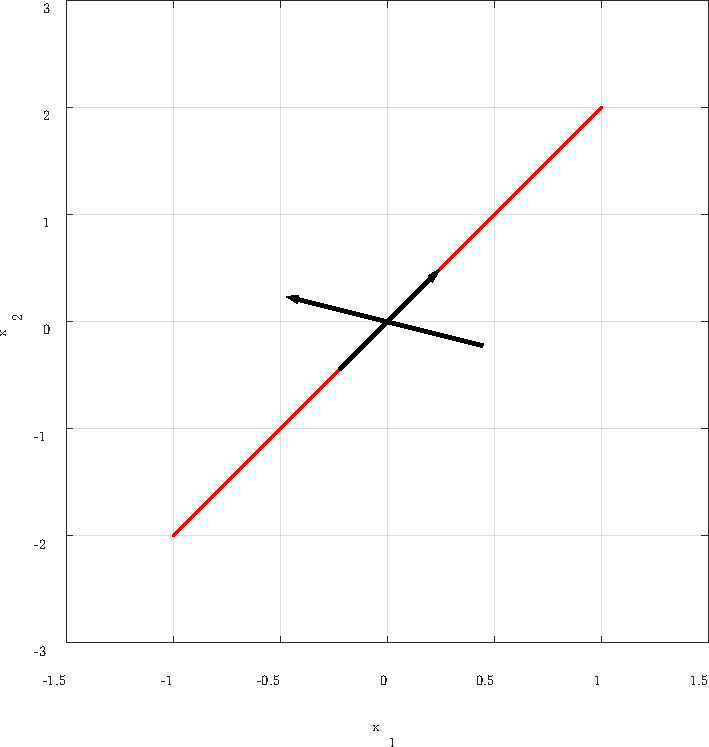
\includegraphics[scale=0.95]{../FIGURES/fig44}
\end{figure}

As we can see, because of the length of the ellipses' minor axis is
$0$, $\lambda_1 \, = \, 0$, the ellipse degenerates in a straight
line. This result match perfectly with the fact I got earlier that
the relation between the random variables $x$ and $y$ is linear,
i.e, $y \, = \, 2\,x ~ \longrightarrow ~ \rho \,=\, 1$.
\end{document}
